\documentclass[twoside, openright, titlepage, fleqn, headinclude, 11pt, a4paper, BCOR5mm, footinclude]{book}

%--------------------------------------------------------------

\usepackage[utf8]{inputenc}
\usepackage[T1]{fontenc}
\usepackage[italian]{babel}
\usepackage[pdftex]{graphicx}
\usepackage[square, numbers]{natbib}
\usepackage[Lenny]{fncychap}
\usepackage[nottoc, notlof, notlot]{tocbibind}
\usepackage[unicode]{hyperref}
\usepackage[fixlanguage]{babelbib}
\usepackage{color, caption, geometry, datetime, url, perpage, afterpage, xfrac, lettrine, yfonts, multirow, wrapfig}

%--------------------------------------------------------------

\newcommand{\mylettrine}[2]{\lettrine[lines=3]{\gothfamily\fontsize{50}{60}\scalebox{2}{#1}}{#2}}
\newcommand{\HRule}{\rule{\linewidth}{0.5mm}}

\newdateformat{monthyear}{\monthname[\THEMONTH] \THEYEAR}

\newtheorem{defi}{Definizione}[chapter]
\newtheorem{teo}{Teorema}[chapter]

\captionsetup{format=hang,font=small}

\MakePerPage{footnote}

\graphicspath{{img/}}

\selectbiblanguage{italian}



%--------------------------------------------------------------

%elimina il numero dalla pagina iniziale delle parti
\makeatletter
\renewcommand{\part}{
	\if@openright
		\cleardoublepage
	\else
		\clearpage
	\fi
	\thispagestyle{empty}	% Original »plain« replaced by »empty«
	\if@twocolumn
		\onecolumn
		\@tempswatrue
	\else
		\@tempswafalse
	\fi
	\null\vfil
	\secdef\@part\@spart
}
\makeatother

%--------------------------------------------------------------

\hypersetup{
	colorlinks,
	citecolor=black,
	filecolor=black,
	linkcolor=black,
	urlcolor=blue
}

%--------------------------------------------------------------

\begin{document}

	\frenchspacing
	\raggedbottom
	\pagenumbering{roman}
	\pagestyle{plain}
	
	\begin{titlepage}
	\begin{center}
		
		
\includegraphics[scale=0.06]{unifi.pdf}\\[0.5cm]
		
		
\includegraphics[scale=0.4]{logo_title.jpg}\\
		\textsc{Facoltà di Scienze Matematiche, Fisiche e Naturali}\\
		\rule{0.8\linewidth}{0.2mm}\\
		\textsc{\footnotesize Corso di Laurea Magistrale in Informatica (classe LM-18)}\\[1.8cm]
		
		\textsc{Anno accademico 2012/2013}\\
		\HRule \\[0.4cm]
		{\huge \bfseries La teoria dell'MP3}\\[0.4cm]
		\HRule \\[0.6cm]
		
		\begin{flushleft}
			\begin{minipage}{0.4\textwidth}
				\emph{Autore:}\\
				Tommaso \textsc{Papini}\\
				tommy39@gmail.com
			\end{minipage}
		\end{flushleft}
		
		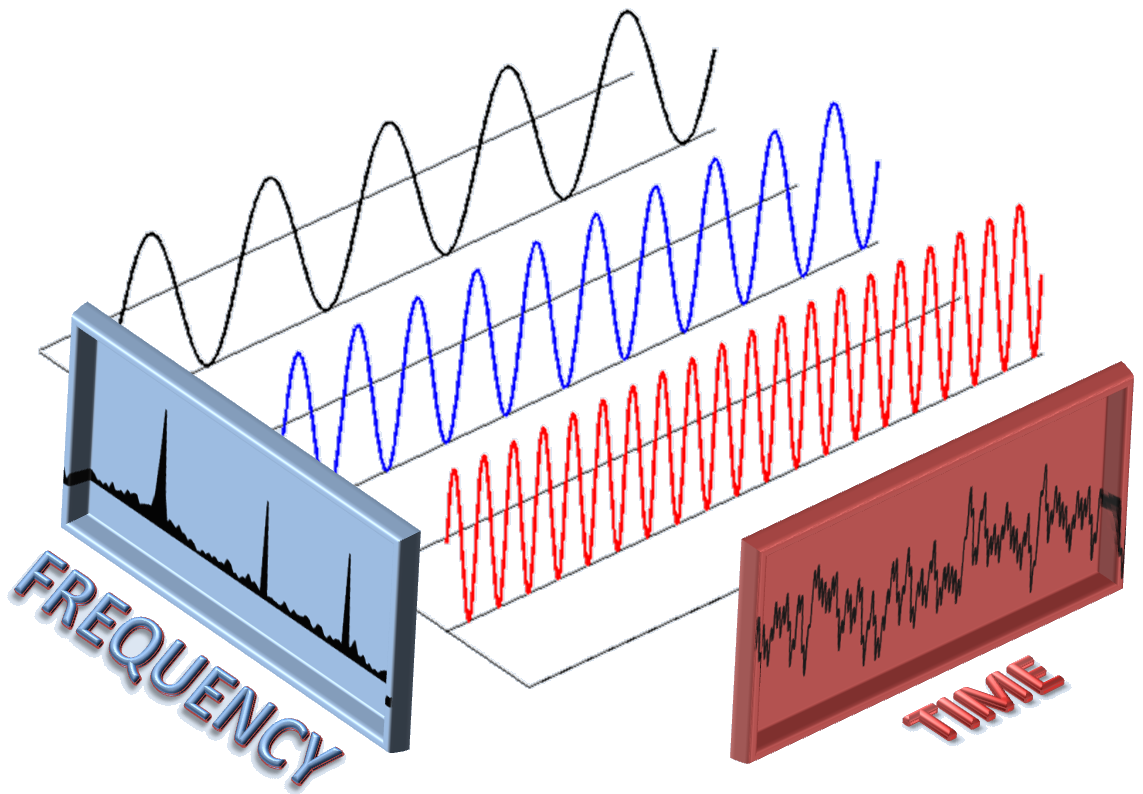
\includegraphics[scale=0.4]{title2.png}
		
		\vfill
		
		{\large \monthyear\today}
		
	\end{center}
\end{titlepage}
	
	\tableofcontents
	\listoffigures
	\listoftables
	
	\cleardoublepage
	\pagenumbering{arabic}
	\pagestyle{headings}
	
	\chapter*{Abstract}
	\addcontentsline{toc}{chapter}{Abstract}
	\markboth{\textsc{\uppercase{Abstract}}}{\textsc{\uppercase{Abstract}}}
	
	\mylettrine{I}{n} questa relazione ci occuperemo di analizzare il formato \textbf{\textit{MP3}} (\textit{MPEG-I Layer III}), ormai ampiamente consolidato in tutto il mondo come formato audio ed efficiente metodo di compressione.\\
	Verrà innanzitutto definito il contesto in cui si viene a trovare l'\textit{MP3}, esponendo brevemente alcuni fondamenti di teoria del suono e raccontando la storia che ha portato all'evoluzione dei formati audio precedenti all'\textit{MP3}.\\
	Quindi verrà analizzato il formato \textit{MP3} stesso, sia come formato di file audio che come metodo di compressione (e decompressione) audio, esponendone le idee di base e le principali tecniche utilizzate.\\
	Infine, verranno proposte alcune note conclusive, non volte ad esporre alcun risultato particolare, ma intese come commentario finale e riassuntivo dell'argomento trattato e della relazione stessa. 
	\part{Breve storia e introduzione} \label{part:intro}
	\chapter{Introduzione} \label{chap:introduzione}
	
	\mylettrine{C}{hiunque} abbia la seppur minima passione per la musica avrà sicuramente sentito parlare, al giorno d'oggi, del formato (o più in generale, della tecnologia) \textit{MP3}. Sicuramente i più sapranno che l'MP3 è un formato audio digitale che permette di memorizzare file audio, come canzoni, utilizzando molto meno spazio rispetto ai precedenti formati, pur mantenendo una buona qualità sonora: molti ricorderanno l'avvento dei primi lettori CD MP3, che permettevano di registrare e riprodurre centinaia di canzoni in un unico CD da 700 MB, al contrario delle massimo 20 canzoni che si potevano masterizzare in qualità CD (di queste differenze di formati e qualità audio parleremo ampiamente più avanti).\\
	La parola MP3 è spesso associata ai concetti di ``Internet'', ``frode'' o ``pirateria informatica'', dal momento che la sua venuta ha dato il via, o comunque incentivato, il download di enormi quantità di dati audio, spesso senza possedere alcuna licenza ed in modo certamente illegale.\\
	\\
	Ma a parte questi aspetti di conoscenza comune, pochi sanno veramente cos'è l'MP3 e come funzioni ed ancor meno sono quelli che si prendono la briga di spiegarlo. Con questo elaborato ci prefiggiamo quindi l'obiettivo di descrivere come e perché è nato l'MP3 e come esso funzioni, senza perdersi troppo nei dettagli tecnici ma fornendo comunque un'idea generale della tecnologia MP3.
	
	\section{Definizioni} \label{sec:definizioni}
		Senza dilungarci troppo nei dettagli, diamo alcune definizioni iniziali che faciliteranno la comprensione di questa relazione.
		
		\begin{defi} \label{defi:mp3}
			L'\emph{\textbf{MP3}} (ovvero \emph{\textbf{M}oving \textbf{P}icture} Expert Group-1/2 Layer \textbf{III}), detto anche \emph{MPEG-1/2 Layer III}, è un algoritmo di compressione audio di tipo \emph{lossy}, sviluppato dal gruppo \emph{MPEG}.
		\end{defi}
		
		Avendo introdotto, nella definizione precedente, il concetto di algoritmo \textit{lossy}, definiamo adesso cos'è un algoritmo di compressione \textit{lossy} e cos'è invece uno \textit{loosless}:
		
		\begin{defi} \label{defi:lossy}
			Un algoritmo di compressione \emph{\textbf{lossy}} è un metodo di codifica che comprime i dati scartandone alcuni. Tramite il processo di decodifica, quindi, non sarà possibile riottenere i dati originali.
		\end{defi}
		
		\begin{defi} \label{defi:loosless}
			Un algoritmo di compressione \emph{\textbf{loosless}} è un metodo di codifica che comprime i dati senza perderne alcuno. Tramite opportuna decodifica sarà quindi possibile ottenere nuovamente i dati originali.
		\end{defi}
		
		Già da queste definizioni possiamo dedurre che l'MP3 è un algoritmo di compressione audio che, comprimendo i dati, scarta alcune informazioni, al fine di rendere il file finale molto più leggero e maneggevole.
		
	\section{Cenni di compressione di dati} \label{sec:cenni_compressione_dati}
		
		Nel 1949 Claude E. Shannon provò, all'interno del suo articolo ``A Mathematical Theory of Communication'', che esiste un limite teorico alla compressione dei dati senza perdere informazione, ovvero comprimendo i dati con algoritmi loosless. Questo limite, detto \textit{tasso d'entropia}, dipende dalla probabilità di trovare determinate sequenze di bit: è possibile comprimere i dati con un tasso di compressione vicino al tasso d'entropia ed è matematicamente impossibile fare meglio.\\
		Per ottenere una maggior compressione dei dati è necessario utilizzare algoritmi lossy e quindi accettare di perdere parte dei dati.\\
		\\
		Di seguito esporremo tre codifiche di tipo loosless molto semplici, una delle quali, come vedremo, utilizzata anche all'interno dell'algoritmo di compressione e decompressione MP3.
		
		\subsection{Run-Length Encoding} \label{subsec:run-length_encoding}
		
			L'algoritmo di compressione loosless \textit{Run-Length Encoding} (o semplicemente \textit{RLE}) consiste nel codificare le varie sequenze di bit consecutivi aventi lo stesso valore come coppie, dove il primo elemento rappresenta il valore di quei bit e il secondo elemento indica il numero di bit che compongono la sequenza, ovvero la lunghezza della sequenza. In Figura \ref{fig:run-length_encoding} possiamo vedere un esempio della codifica RLE. Questa codifica è ideale per dati con lunghe sequenze di bit identici (quindi sconsigliato per dati casuali).
			
			\begin{figure}[h!]
				\centering
					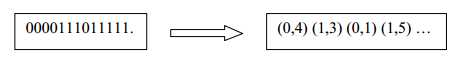
\includegraphics[scale=1]{run-length_encoding.png}
				\caption{Algoritmo di compressione Run-Length Encoding.}
				\label{fig:run-length_encoding}
			\end{figure}
			
		\subsection{Move-To-Front} \label{subsec:move-to-front}
			
			La codifica \textit{Move-To-Front} (o \textit{MTF}) si basa sul concetto di entropia ed infatti è ottimizzata quando la lettura di un carattere aumenta le probabilità di trovare lo stesso carattere subito dopo.\\
			L'algoritmo inizia codificando le lettere dell'alfabeto secondo l'ordine usuale (da 0 a 25). Quindi ogni carattere che viene incontrato viene spostato in cima alla lista. In generale, elementi in cima alla lista vengono codificati con meno bit, mentre quelli verso il fondo richiedono più bit.\\
			\\
			Se ad esempio prendiamo la parola ``BANANAAA'', la codifica MTF di questa parola sarà quella in Tabella \ref{tab:move-to-front}.
			
			\begin{table}[h!]
				\centering
				\begin{tabular}{|l|l|c|}
					\multicolumn{1}{c}{\textbf{Sequenza}} & \multicolumn{1}{c}{\textbf{Codifica}} & \multicolumn{1}{c}{\textbf{Lista}}\\
					\hline
					b & 1 & abcdefghijklmnopqrstuvwxyz\\
					\hline
					ba & 1, 1 & bacdefghijklmnopqrstuvwxyz\\
					\hline
					ban & 1, 1, 13 & abcdefghijklmnopqrstuvwxyz\\
					\hline
					bana & 1, 1, 13, 1 & nabcdefghijklmopqrstuvwxyz\\
					\hline
					banan & 1, 1, 13, 1, 1 & anbcdefghijklmopqrstuvwxyz\\
					\hline
					banana & 1, 1, 13, 1, 1, 1 & nabcdefghijklmopqrstuvwxyz\\
					\hline
					bananaa & 1, 1, 13, 1, 1, 1, 0 & anbcdefghijklmopqrstuvwxyz\\
					\hline
					bananaaa & 1, 1, 13, 1, 1, 1, 0, 0 & anbcdefghijklmopqrstuvwxyz\\
					\hline
				\end{tabular}
				\caption{Algoritmo di compressione Move-To-Front.}
				\label{tab:move-to-front}
			\end{table}
		
		\subsection{Codifica di Huffman} \label{subsec:codifica_huffman}
			
			Il concetto di entropia viene ampiamente applicato anche alla codifica di Huffman che, come vedremo più avanti, viene utilizzata all'interno dell'algoritmo di compressione MP3. L'idea che sta alla base della codifica di Huffman è quella di codificare con meno bit i caratteri più frequenti. La probabilità di incontrare determinati caratteri dev'essere determinata a priori (ad esempio analizzando i dati che si vogliono comprimere). Successivamente, in base alle probabilità calcolate, si assegnano codifiche più corte ai caratteri più frequenti e si memorizzano le associazioni carattere-codifica in una tabella, detta \textit{tabella di Huffman}, necessaria per la successiva decodifica dei dati. Come possiamo vedere in Figura \ref{fig:huffman}, la tabella di Huffman può essere rappresentata anche come un albero binario.
			
			\begin{figure}[h!]
				\centering
					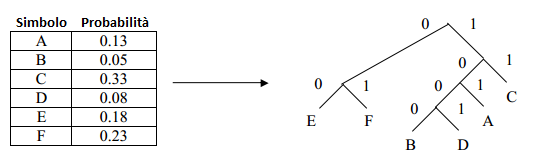
\includegraphics[scale=1]{huffman.png}
				\caption{Codifica di Huffman.}
				\label{fig:huffman}
			\end{figure}
		
	\chapter{Cenni di teoria del suono} \label{chap:teoria_suono}
	
	\mylettrine{I}{ntuitivamente}, prima di poter parlare di algoritmi di compressione audio, e quindi di MP3, sarà necessario innanzitutto definire cos'è il suono e come si comporta. In questo capitolo verranno quindi presentati alcuni concetti fondamentali di teoria del suono, sia dal punto di vista fisico (onde e tutto ciò che ne concerne) che dal punto di vista informatico (campionamento e sintesi).
	
	\section{Il suono come onda} \label{sec:suono_onda}
		
		\begin{defi} \label{defi:suono}
			Il \emph{\textbf{suono}} è un'\emph{onda meccanica}, ovvero un'\emph{onda di pressione} che si propaga attraverso un mezzo.
		\end{defi}
		
		Questa definizione che abbiamo appena dato sul suono è molto chiara e concisa: il suono è un'onda. Ma non una qualsiasi onda. Il suono è un'onda di pressione, ovvero non è nient'altro se non l'oscillazione (movimento ``avanti-indietro'', in parole povere) del mezzo in cui si propaga, che può essere solido o fluido. Il timpano umano è infatti una membrana sottilissima volta a captare queste oscillazioni presenti attorno a noi; sarà poi il cervello che tradurrà i movimenti della membrana in informazioni utili, interpretandole come quello che noi chiamiamo suono.\\
		Come tutte le onde, anche il suono avrà quindi tutta una serie di attributi caratteristici, quali:
		\begin{itemize}
			\item \textbf{periodo}: minimo intervallo di tempo dopo il quale i valori dell'onda si ripetono ($s$, secondi);
			\item \textbf{frequenza}: numero di oscillazioni per unità di tempo ($Hz$, hertz);
			\item \textbf{lunghezza d'onda}: minima distanza dopo la quale  i valori dell'onda si ripetono($m$, metri);
			\item \textbf{numero d'onda}: numero di oscillazioni per unità di lunghezza ($m^{-1}$, metri alla meno uno);
			\item \textbf{ampiezza}: misura i cambiamenti dell'onda all'interno di uno stesso periodo (varia);
				\begin{itemize}
					\item \textit{ampiezza picco-a-picco}: massimo scarto tra una cresta (punto di massimo dell'onda) e la valle (punto di minimo) successiva;
					\item \textit{ampiezza a picco}: massimo valore assoluto dell'onda;
					\item \textit{ampiezza RMS} (root mean square): scarto quadratico medio dell'ampiezza.
				\end{itemize}
			\item \textbf{velocità}: velocità con cui l'onda si propaga nel mezzo ($\sfrac{m}{s}$, metri al secondo).
		\end{itemize}
		
		\begin{figure}[h!]
			\centering
				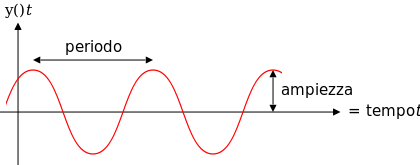
\includegraphics[scale=0.7]{periodo_ampiezza.png}
			\caption{Periodo e ampiezza di un'onda periodica.}
			\label{fig:periodo_ampiezza}
		\end{figure}
		
		\begin{figure}[h!]
			\centering
				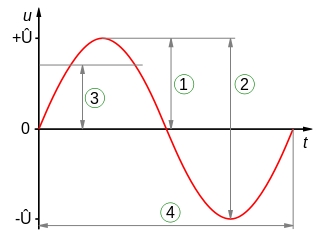
\includegraphics[scale=0.75]{ampiezze.png}
			\caption[Diversi tipi di ampiezze.]{Diversi tipi di ampiezze: ampiezza a picco (1), ampiezza picco-a-picco (2) e ampiezza RMS (3).}
			\label{fig:ampiezze}
		\end{figure}
		
		Come è facile dedurre, \textit{periodo} e \textit{frequenza} sono uno l'inverso dell'altro, come anche \textit{lunghezza d'onda} e \textit{numero d'onda}. L'unità di misura dell'ampiezza dipende dal tipo d'onda che si sta analizzando: se si tratta di corrente elettrica può rappresentare un voltaggio ($V$, volt), una corrente ($A$, ampere) o la potenza ($W$, watt), mentre se parliamo di onde sonore l'ampiezza può rappresentare la forza dell'onda di pressione (\textit{dB}, decibel), oppure il movimento oscillatorio stesso, con 0 punto di quiete e -1 ed 1 limiti, rispettivamente, inferiore e superiore. La velocità d'onda è invece calcolata come $v=\sfrac{\lambda}{p}=\lambda\cdot f$, dove $\lambda$ è la lunghezza d'onda, $p$ il suo periodo ed $f$ la sua frequenza. La velocità del suono a 20 ${}^\circ C$ nell'aria al livello del mare è circa 343 $\sfrac{m}{s}$, ma come per molte altri tipi di onda la sua velocità varia a seconda di molti fattori, come natura del mezzo, temperatura, densità, ecc\dots.
	
	\section{Percezione del suono} \label{sec:percezione}
	
		Avendo definito il suono come un'onda, possiamo affermare che in natura esistono un'infinità di suoni diversi, generati da altrettante frequenze caratteristiche. L'orecchio umano, tuttavia, non è in grado di percepire tutte le frequenze esistenti in natura: in generale, l'uomo riesce a percepire tutte le frequenze che vanno dai 20 \textit{Hz} ai 20 \textit{kHz} (20mila \textit{Hz}). Ovviamente, ci sono eccezioni e casi particolari di persone che affermano di riuscire a percepire e distinguere anche frequenze al di fuori di questo range. Inoltre, l'uomo non percepisce tutte le frequenze allo stesso modo: più ci si avvicina ai limiti del range di udibilità, più sarà difficile percepire tale suono. Infatti le frequenze che meglio possiamo sentire sono quelle tra i 2 e i 4 \textit{kHz} \cite{raissi}.\\
		A tal proposito, la Figura \ref{fig:ath} rappresenta la \textit{soglia assoluta di udibilità} (in inglese, \textit{absolute threshold of hearing}) per un uomo medio a 20, 40 e 60 anni, ovvero qual'è la minima intensità che ogni frequenza deve avere per essere percepita dall'uomo. In altre parole, tutto ciò che l'uomo non sente è rappresentato dall'area sottesa dal grafico in Figura \ref{fig:ath}.
		
		\begin{figure}[h!]
			\centering
				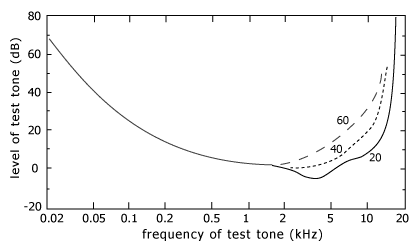
\includegraphics[scale=1]{ath.png}
			\caption[Soglia assoluta di udibilità.]{Soglia assoluta di udibilità per un uomo medio a 20, 40 e 60 anni.}
			\label{fig:ath}
		\end{figure}
		
		L'uomo, quindi, non è una macchina, in quanto il suo orecchio e il suo cervello non sono strumenti perfetti. È nata infatti negli anni la disciplina detta \textit{psicoacustica}, che si occupa di studiare non tanto il suono in sé dal punto di vista fisico, ma come esso viene percepito dall'uomo. Della psicoacustica sentiremo parlare più avanti quando entreremo nel merito dell'MP3, in quanto essa costituisce uno dei principi cardine che stanno alla base della tecnologia MP3.
		
	\section{Sintesi e Campionamento} \label{sec:campionamento_sintesi}
	
		Abbiamo detto che il suono è un'onda di pressione, ovvero il movimento oscillatorio (``avanti-indietro'') del mezzo nel quale si propaga. Infatti tutti i suoni sono prodotti dal movimento, più o meno rapido, di uno o più corpi, il quale genera questa catena di oscillazioni, producendo il suono stesso.
		
		\subsection{Sintesi} \label{subsec:sintesi}
		
			Come viene riprodotto, allora, artificialmente un suono? Secondo quanto detto, abbiamo bisogno di un corpo che faccia a comando questo movimento oscillatorio. Non solo, è necessario anche che il movimento ``avanti-indietro'' che questo corpo esegue abbia la stessa frequenza del suono che vogliamo riprodurre, ovvero che esegua lo stesso numero di oscillazioni nell'unità di tempo.\\
			\\
			L'oggetto di cui stiamo parlando è detto \textit{speaker}, o più comunemente \textit{altoparlante}. Uno speaker è formato da un elettromagnete che, a seconda dell'intensità della corrente elettrica che lo attraversa, si sposterà avanti o indietro rispetto alla posizione di quiete. La gestione dello speaker avviene tramite una \textit{scheda audio} (o \textit{soundcard} in inglese), ovvero un DAC (\textit{Digital-to-Analog Converter}) che trasforma un numero digitale in input in un segnale elettrico in output. Se si utilizza la convenzione prima esposta (0 = stato di quiete, -1 = tutto indietro, 1 = tutto avanti) possiamo allora fornire alla scheda audio una serie di valori nel tempo, in modo da far muovere lo speaker avanti e indietro. Se rappresentassimo questo movimento in funzione del tempo, otterremmo proprio i ben noti grafici delle onde sonore, come quelli nelle Figure \ref{fig:periodo_ampiezza} e \ref{fig:ampiezze}. Ad esempio per riprodurre la nota La, che ha una frequenza di 440 \textit{Hz} \cite{mtu}, lo speaker dovrà eseguire 440 oscillazioni ``avanti-indietro'' ogni secondo.
			
		\subsection{Campionamento} \label{subsec:campionamento}
		
		\begin{figure}[h!]
			\centering
				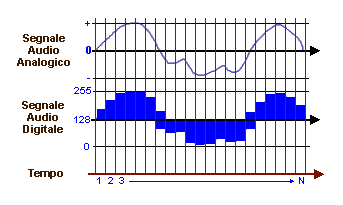
\includegraphics[scale=1]{campione.png}
			\caption{Campionamento di un segnale audio analogico.}
			\label{fig:campione}
		\end{figure}
		
		Si osservi che, per quanto detto prima, per oscillazione si intende un intero movimento ``avanti-indietro'', ovvero un intero periodo, quindi affinché il suono della nota La venga prodotto correttamente, lo speaker dovrà effettuare 440 movimenti in avanti e 440 movimenti indietro e sarà quindi necessario fornire alla scheda audio l'informazione su questi 880 movimenti totali. Il fatto di richiedere il doppio di informazione rispetto al numero di oscillazioni al secondo è noto come \textit{Teorema del campionamento di Shannon-Nyquist}. Prima di parlare di questo importante teorema, introduciamo due concetti chiave del campionamento:
		
		\begin{defi} \label{defi:sampling_frequency}
			La \emph{\textbf{sampling frequency}} (o \emph{frequenza di campionamento}) è il numero di volte in cui viene misurato (o campionato) un segnale audio esterno in un determinato intervallo di tempo.
		\end{defi}
		
		\begin{defi} \label{defi:bit_depth}
			La \emph{\textbf{bit depth}} (o \emph{profondità di bit}) indica il numero di bit riservati alla memorizzazione di ogni campione (o sample).
		\end{defi}
		
		Un microfono, in linea di massima, è sostanzialmente un altoparlante al contrario: una membrana collegata ad un elettromagnete si muove secondo i suoni esterni, assecondandone i movimenti. Ogni $\sfrac{1}{f}$ secondi (con $f$ frequenza di campionamento) viene misurata la posizione di questa membrana rispetto alla posizione di quiete. Questa misura prende il nome di \textit{campione} (o \textit{sample}) e ognuno di questi campioni verrà registrato in memoria utilizzando un numero di bit definito dalla bit depth. Una volta registrati abbastanza campioni, effettuare la sintesi tramite scheda audio e speaker sarà semplice: verrà effettuata una semplice interpolazione tra i sample registrati e i valori della funzione risultante verrano dati in pasto alla scheda audio, che azionerà lo speaker di conseguenza.\\
		Ovviamente, una maggiore sampling frequency permette di avere campionamenti più fitti e quindi una riproduzione più accurata del suono registrato. Analogamente, più bit si riservano per i campioni, minore sarà l'errore commesso su ogni misura (detto \textit{errore di quantizzazione}), rendendo ancora una volta la registrazione più accurata. Tuttavia, avere più sample e/o avere sample più voluminosi (come quantità di bit) andrà a incidere negativamente sulle dimensioni totali della registrazione risultante, rendendo, in casi estremi, il file finale eccessivamente grande.\\
		Possiamo quindi trovare un compromesso tra dimensioni del file e qualità audio? Come vedremo più avanti, il punto di forza dell'MP3 sta proprio nell'aver definito un modo di memorizzare i file audio che permetta sia di godere di un'ottima qualità audio che, allo stesso tempo, di mantenere le dimensioni del file ridotte.\\
		
		\begin{figure}[h!]
			\centering
				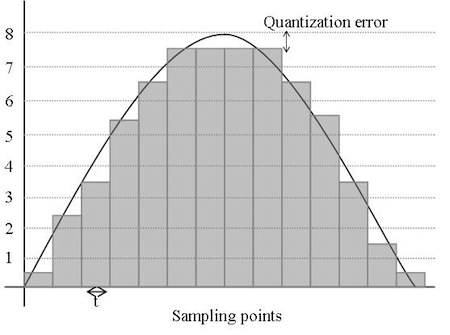
\includegraphics[scale=1]{quantization.jpg}
			\caption{Campionamento ed errore di quantizzazione.}
			\label{fig:quantization}
		\end{figure}
		
		\begin{figure}[h!]
			\centering
				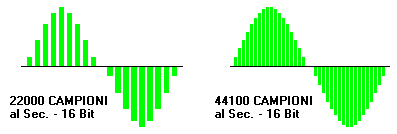
\includegraphics[scale=1]{sampling_22_441.png}
			\caption[Uso di differenti sample frequency.]{Uso di differenti sampling frequency: all'aumentare della sampling frequency aumenta la fedeltà del file audio ma anche le dimensioni complessive.}
			\label{fig:sampling_22_441}
		\end{figure}
		
		Il Teorema del campionamento di Shannon-Nyquist serve a mettere in relazione la frequenza di campionamento con la frequenza di output ottenuta dalla sintesi:
		
		\begin{teo}[Shannon-Nyquist] \label{teo:shannon_nyquist}
			Per poter correttamente riprodurre un segnale audio, come minimo devono essere misurati due campioni per ogni periodo della sua onda caratteristica.
		\end{teo}
		
		Quindi come dicevamo prima, se vogliamo correttamente riprodurre una nota La (440 \textit{Hz}), avremmo bisogno di una frequenza di campionamento di almeno 880 \textit{Hz}. Viceversa, campionando con una frequenza fissata, non sarà possibile riprodurre tutte le frequenze maggiori della metà della sampling frequency (noto come \textit{limite di Nyquist}).\\
		La ``qualità CD'', infatti, è caratterizzata da una sampling frequency di 44.1 \textit{kHz}, il che significa che verranno scartate tutte le frequenze al di sopra dei 22.05 \textit{kHz}. Questo valore non è casuale: 22.05 \textit{kHz} è poco sopra il limite superiore di udibilità dell'uomo (20 \textit{kHz}). In parole povere, registrare frequenze più alte sarebbe soltanto uno spreco di spazio, in quanto non verrebbero comunque udite dall'uomo.\\
		\\
		Se la frequenza di campionamento non è abbastanza elevata, alcuni campioni si potrebbero sovrapporre in frequenza, dando origine al fenomeno (negativo) detto \textit{aliasing}: l'aliasing rende impossibile ricostruire parte del segnale originale a partire dai suoi campioni (come formalizzato dal Teorema di Shannon-Nyquist). L'aliasing si elimina aumentando la frequenza di campionamento. Se il segnale di input non è a banda limitata, allora si filtra prima attraverso un filtro passa-basso, detto \textit{filtro anti-aliasing}.
	\chapter{Storia: dal PCM all'MP3} \label{chap:storia}
	\mylettrine{A}{vevamo} detto, nel capitolo introduttivo, che l'MP3 è sì un formato di file audio, ma anche che con MP3 si intende principalmente un algoritmo di compressione audio (di tipo lossy). Viene allora spontaneo chiedersi a che tipo di formato audio si applichi la compressione MP3, ovvero che formato audio era predominante prima dell'arrivo dell'MP3.
	
	\section{PCM} \label{sec:pcm}
		La risposta a queste domande è racchiusa nella sigla \textit{PCM}. \textit{PCM}, che sta per \textit{\textbf{P}ulse \textbf{C}ode \textbf{M}odulation} (ovvero \textit{Modulazione a Codice di Impulsi}), è sostanzialmente il metodo di campionamento descritto nel Capitolo \ref{chap:teoria_suono}: per registrare e memorizzare un segnale audio esterno si eseguono delle misure a intervalli di tempo regolari (dettati dalla sampling frequency), quindi si quantizzano i sample ottenuti (ovvero si mappano in valori discreti) ed infine si digitalizzano (ovvero si codifica ogni campione in codice binario).\\
		In sostanza, il metodo PCM tende a catturare un segnale audio esterno registrandone e memorizzandone una serie di valori, in modo da poter approssimare e ricostruire l'onda caratteristica ogni qual volta si voglia riprodurre quel suono.
		
		\subsection{Il problema delle dimensioni} \label{subsec:dimensioni}
			Ovviamente la PCM può operare a diversi valori di sampling frequency e di bit depth, anche se l'accoppiata più famosa è quella relativa alla qualità CD, ovvero 44.1 \textit{kHz} di sampling frequency e 16 bit come bit depth.\\
			Questo significa che ogni secondo vengono registrati 44100 campioni, ognuno dei quali grande 16 bit, ovvero 88200 byte al secondo \footnote{Calcolato come: $(44100\cdot 16)/8=88200\mbox{ byte }$.}. Questo valore raddoppia se l'audio registrato è stereo (una registrazione per il canale sinistro ed una per il canale destro). Con queste premesse, è facile vedere che un minuto di audio stereo in PCM occupa poco più di 10 MB. Quindi un normale CD da 700 MB può contenere soltanto 70 minuti di audio in questo formato, che corrispondono a circa 20 canzoni \footnote{Considerando una durata media per canzone di 3.5 minuti.}\\
			\\
			Fintanto che si parla di CD audio, queste limitazioni non presentano un vero problema. Tuttavia quando si parla di applicazioni, che registrano su computer grandi quantità di audio, e specialmente di applicazioni su Web, per le quali è necessario scambiare file audio a grande velocità, le dimensioni dei file iniziano a pesare e a diventare un problema non indifferente.\\
			\\
			Un primo approccio per diminuire le dimensioni dei file audio è quello di diminuire la sampling frequency: meno campioni significa meno spazio necessario. Se dimezziamo la frequenza di campionamento, allora avremo esattamente la metà dei campioni e quindi un file grande la metà rispetto all'originale. Tuttavia, per il Teorema di Shannon-Nyquist (Teorema \ref{teo:shannon_nyquist} a pagina \pageref{teo:shannon_nyquist}), sappiamo che il limite superiore delle frequenze riproducibili è dato dalla metà della sampling frequency, quindi dimezzando quest'ultima dimezzeremo di fatto anche il limite di Nyquist, scartando metà frequenze di quelle che prima venivano registrate. Se ad esempio dimezziamo la sampling frequency della qualità CD, da 44.1 \textit{kHz} a 22.05 \textit{kHz}, avremo che verranno scartate non più le frequenze maggiori di 22.05 \textit{kHz}, ma tutte quelle maggiori di 11.025 \textit{kHz}. Mentre quelle maggiori di 22 \textit{kHz} non ci interessano più di tanto (per via del range di udibilità umano 20 \textit{Hz} - 20 \textit{kHz}) quelle comprese tra 11.025 e 22.05 \textit{kHz} invece sono frequenze importanti, in quanto udibili dall'uomo. Perdere queste frequenze risulterebbe, inevitabilmente in una perdita di qualità del segnale audio.\\
			\\
			Un secondo approccio è invece quello di diminuire la bit depth, ovvero di assegnare meno bit ad ogni campione registrato. Diminuendo i bit per ogni sample ovviamente diminuiscono anche le dimensioni totali, ma aumenta anche l'errore di quantizzazione, in quanto meno bit devono essere usati per approssimare una grandezza continua. In questo frangente, tuttavia, le perdite relative alla diminuzione di bit depth sono molto più gravi rispetto alla diminuzione della sampling frequency. Infatti, dimezzando la bit depth di ogni sample le dimensioni totali saranno sì dimezzate, tuttavia la qualità del suono risultante sarà più che dimezzata. Se pensiamo ad un campionamento a 16 bit, ricaviamo che ogni sample può assumere uno di 65536 ($2^{16}$) diversi valori, che è come dire che la misura ottenuta può essere rappresentata utilizzando 65536 ``sfumature'' diverse. Tuttavia utilizzando 8 bit per ogni sample, abbiamo che ogni campione potrà assumere uno di 256 ($2^8$) possibili valori, che è molto meno della metà.\\
			Diminuire la bit depth porta quindi ad un aumento esponenziale degli errori di quantizzazione, diminuendo il cosiddetto \textit{rapporto segnale/rumore}.
			
	\section{MP3}
		Con queste premesse, la \textit{ISO} (\textit{International Standards Organization}) e la \textit{IEC} (\textit{International Electrothecnical Commision}) formarono il gruppo \textit{MPEG} (ovvero \textit{Moving Picture Experts Group}), nella speranza di definire uno standard mondiale per la codifica di video e audio di alta qualità. In particolare, si erano proposti come obiettivo quello di definire un metodo di codifica audio e video che permettesse la scrittura e la lettura da un generico dispositivo capace di fornire 1.5 Mbit al secondo (come i ben noti CD).\\
		Un punto cruciale divenne allora la compressione di questi dati, in quanto la lettura e scrittura di dati audio e video non compressi richiederebbe molto di più di 1.5 Mbit al secondo, infatti il solo audio codificato tramite PCM richiede un bitrate di 1.4 \textit{Mbps} per la sua riproduzione \footnote{Calcolato come $44.1\mbox{ \textit{kHz}}\cdot 16\mbox{ \textit{bit}}\approx 0.7\mbox{ \textit{Mbps}}$ per audio mono, $1.4\mbox{ \textit{Mbps}}$ per audio stereo (il doppio).}.
		
		\subsection{Lo standard MPEG 1} \label{subsec:mpeg1}
		
			Lo standard \textit{MPEG 1}, riguardante appunto la compressione di video e dell'audio associato, fu pubblicato dal gruppo MPEG nel 1993, sotto il nome di \textit{ISO/IEC 11172}. La parte relativa alla compressione audio dell'MPEG 1 fu suddivisa in tre \textit{Layer}, o \textit{livelli}: questi livelli aggiungono, ognuno, nuovi meccanismi di compressione audio, rendendo la compressione stessa più complessa ed efficiente ad ogni livello. Inoltre questi layer sono retrocompatibili, ovvero un decoder costruito per il Layer 3 riesce a decodificare anche file codificati con il Layer 2 e con il Layer 1. Quello che noi oggi chiamiamo MP3 è, di fatto, tutto l'algoritmo di compressione dell'MPEG 1 Layer 3.\\
			Successivamente, nel 1995, una seconda versione dello standard MPEG venne pubblicata, chiamata comunemente \textit{MPEG 2} e formalmente \textit{ISO/IEC 13818}. Ai fini delle tecniche caratteristiche dell'MP3 è indifferente parlare di MPEG 1 o 2, infatti spesso ci si riferisce all'MP3 come \textit{MPEG 1/2 Layer 3}.\\
			\\
			Ogni layer dello standard MP3 aggiunge complessità all'algoritmo, riuscendo ad ottenere una compressione sempre più efficace. In Tabella \ref{tab:bitrate} possiamo vedere i fattori di compressione MPEG 1 rispetto alla codifica PCM e il bitrate richiesto per la riproduzione di un file audio all'aumentare della complessità di compressione.
			
			\begin{table}[h!]
				\centering
				\begin{tabular}{|c|c|c|}
					\multicolumn{1}{c}{\textbf{Codifica}} & \multicolumn{1}{c}{\textbf{Rapporto}} & \multicolumn{1}{c}{\textbf{Bitrate richiesto}}\\
					\hline
					PCM (qualità CD) & 1:1 & 1.4 \textit{Mbps}\\
					\hline
					Layer 1 & 4:1 & 384 \textit{kbps}\\
					\hline
					Layer 2 & 8:1 & 192 \textit{kbps}\\
					\hline
					Layer 3 & 12:1 & 128 \textit{kbps}\\
					\hline
				\end{tabular}
				\caption{Bitrate richiesti per le codifiche MPEG 1.}
				\label{tab:bitrate}
			\end{table}
			
			Si ha quindi che la codifica MP3 riesce a diminuire le dimensioni di un file audio, codificato con la PCM, di un fattore 12, diminuendo notevolmente le dimensioni originali, senza tuttavia intaccarne notevolmente la qualità, grazie ai principi della psicoacustica che vedremo più avanti.
			
		\subsection{Libertà d'implementazione} \label{subsec:libertà_implementazione}
			
			Le specifiche dello standard ISO 11172-3 (ovvero dell'MP3) definiscono come dev'essere strutturato e interpretato un file \texttt{.mp3} e come deve avvenire la decodifica di quest'ultimo. Questo è ciò che rende l'MP3 uno standard internazionale: un file \texttt{.mp3}, infatti, potrà essere decodificato da qualsiasi decoder MP3.\\
			Tuttavia, molte fasi di codifica e dettagli implementativi non sono specificati nello standard ISO, lasciando agli sviluppatori una discreta libertà di scelta per quanto riguarda le varie parti dell'encoder. In altre parole, lo standard definisce soltanto cosa si deve ottenere dalla codifica, ma non come eseguire la codifica stessa: diversi sviluppatori possono utilizzare tecniche diverse per ottenere lo stesso risultato, o addirittura impiegare nuove tecniche che migliorano/velocizzano il processo di codifica.\\
			Il processo di decodifica è invece già più standardizzato, anche se molti dettagli implementativi vengono lasciati allo sviluppatore finale.
			
		\subsection{Alcuni dettagli tecnici} \label{subsec:dettagli_tecnici} 
			
			Concludiamo esponendo alcuni dettagli tecnici dello standard MP3.\\
			\\
			Innanzitutto parliamo di \textit{bitrate}. Il \textit{bitrate} (letteralmente \textit{tasso di bit}) indica quanti bit di memoria sono dedicati ad ogni secondo del segnale audio, ovvero quanti bit al secondo devono essere letti per la sua riproduzione. Ovviamente più bit al secondo implica una maggior qualità del suono ma anche maggiori dimensioni del file. Lo standard MP3 prevede bitrate dagli 8 \textit{kbps} fino ai 320 \textit{kbps}, anche se il valore più utilizzato è 128 \textit{kbps}.\\
			In linea di massima, lo standard MPEG 1 Layer 3 definisce due tipologie di bitrate: il \textit{bitrate costante} (\textit{Constant BitRate}, \textit{CBR}) e il \textit{bitrate variabile} (\textit{Variable BitRate}, \textit{VBR}). Con il \textbf{bitrate costante} si assegna lo stesso numero di bit a ogni secondo del file audio. Tuttavia molte registrazioni (ad esempio canzoni) variano spesso di complessità, passando da momenti in cui suonano molti strumenti (e quindi più bit sono richiesti per avere una buona fedeltà) ad altri più semplici (in cui basterebbero pochi bit al secondo). Con il \textbf{bitrate variabile} si possono invece assegnare a diverse parti della canzone (dette \textit{frame}, come vedremo più avanti) una quantità diversa di bit, a seconda della complessità del segnale.\\
			\\
			La qualità finale del file \texttt{.mp3} è anche data dalla sampling frequency (come già avevamo visto per la PCM): più campioni al secondo significa una più alta qualità audio, ma anche un file più voluminoso. Lo standard MP3 prevede la codifica a 32, 44.1 o 48 \textit{kHz}.\\
			\\
			Infine, un file \texttt{.mp3} avrà una delle seguenti \textit{modalità di canale} (\textit{channel mode}):
			\begin{itemize}
				\item canale singolo (mono);
				\item canale doppio;
				\item stereo;
				\item joint stereo.
			\end{itemize}
			Il \textit{canale singolo} (o \textit{mono}) è il più semplice di tutti e prevede un singolo flusso di dati audio. Il \textit{canale doppio} prevede invece due canali singoli indipendenti (uno destro ed uno sinistro). La modalità \textit{stereo} prevede invece due canali non indipendenti, in quanto i bit per ogni canale posso essere ripartiti tra i due (se ad esempio in un certo momento il segnale sinistro è più complesso di quello destro, si possono prendere alcuni bit di quest'ultimo). Con \textit{joint stereo} si intende invece una modalità che tenta di ottimizzare la codifica dei due canali eliminando le ridondanze tra questi. Esistono due tecniche per il joint stereo: \textit{mid/side stereo} (o \textit{MS stereo}) e \textit{intensity stereo}. Mid/side stereo è composto da due canali: \textit{mid}, che rappresenta le parti in comune tra canale destro e sinistro, e \textit{side}, che rappresenta le differenze tra canale destro e sinistro. In intensity stereo invece le frequenze più alte vengono sommate tra loro, in modo da riuscire a trasmettere tutto in un unico canale. MS stereo è una tecnica loosless, mentre intensity stereo è una tecnica lossy, anche se le inconsistenze introdotte sono spesso non percepibili all'orecchio umano.
			
	\part{MP3} \label{part:mp3}
	\chapter{Introduzione all'MP3} \label{chap:introduzione_mp3}
	
	\mylettrine{A}{bbiamo} visto, nei capitoli precedenti, che il metodo di campionamento della PCM aveva come obiettivo quello di riprodurre, il più fedelmente possibile, l'onda caratteristica di un segnale audio esterno. Tuttavia questo approccio racchiude in sé un'assunzione implicita, ovvero che sia necessario disporre dell'onda caratteristica per poter riprodurre correttamente un segnale audio. Quest'assunzione nasce sostanzialmente da una scarsa conoscenza della percezione del suono da parte dell'orecchio e del cervello umano.
	
	\section{Codifica percettiva} \label{sec:codifica_percettiva}
		Il problema di fondo è che l'orecchio ed il cervello umano sono  ``strumenti'' imperfetti, che non captano il suono in maniera perfetta e assoluta per come è, ma lo interpretano secondo una serie di fattori. Un esempio è rappresentato dalla soglia assoluta di udibilità umana (in Figure \ref{fig:ath}). È stato dimostrato, inoltre, che raddoppiare l'ampiezza di un segnale audio non corrisponde ad un raddoppiamento dell'effettivo volume percepito. In generale, esistono molti aspetti del suono che l'orecchio ed il cervello umano semplicemente trascurano, accentuando alcune proprietà dei suoni esterni anziché percepire tutto in modo assoluto.\\
		\\
		Come già accennato, la disciplina che si occupa dello studio della percezione del suono prende il nome di \textit{psicoacustica} ed assume un ruolo chiave nella tecnologia MP3.\\
		L'idea di base dell'MP3 è la seguente: se alcune caratteristiche del suono non vengono comunque percepite dall'uomo, perché sprecare spazio inutilmente cercando di riprodurre tutta l'onda caratteristica? Sarebbe molto più intelligente cercare di memorizzare e riprodurre soltanto quelle parti del suono che effettivamente verrano percepite.\\
		Infatti quello che fa l'MP3 è proprio di selezionare le caratteristiche più rilevanti di un certo suono ed assegnargli una maggiore priorità, in modo da riprodurle più fedelmente a scapito di caratteristiche meno rilevanti o superflue. Si potrebbe dire che, mentre la PCM tenta di catturare un segnale audio ``per come è'', l'MP3 tenta di catturarlo ``per come suona''.\\
		\\
		Risulta allora necessario definire cosa è rilevante per l'orecchio umano e cosa non lo è: queste informazioni costituiscono il cosiddetto \textbf{modello psicoacustico}, che definisce quanto e quali parti del suono sono rilevanti.\\
		Prima di entrare nel dettaglio del modello psicoacustico, è necessario definire due concetti chiave: \textit{ridondanza} e \textit{irrilevanza}, che suddividono in due categorie distinte tutte quelle informazioni del suono considerate non necessarie per l'uomo, o comunque eliminabili senza perdere troppo in termini di qualità audio.\\
		Abbiamo già parlato di \textbf{ridondanza} quando abbiamo visto il metodo PCM ed abbiamo parlato del limite di Nyquist: nella qualità CD (frequenza di campionamento di 44.1 \textit{kHz}) tutte le frequenze maggiori di 22.05 \textit{kHz} vengono automaticamente considerate ridondanti, e quindi scartate. Si potrebbe aumentare la sampling frequency, per catturare più alte frequenze, ma il limite in questione non verrebbe eliminato, ma soltanto spostato più in alto. In altre parole, la ridondanza è un concetto onnipresente nel mondo digitale.\\
		L'\textbf{irrilevanza}, invece, è un concetto molto più complesso, che descrive tutte quelle caratteristiche di un'onda sonora che sono prive di senso in termini di percezione umana. Tutte queste caratteristiche, irrilevanti per l'uomo, verranno descritte in un opportuno modello psicoacustico e quindi eliminate (o ridotte di dimensioni) dal file audio finale, diminuendo le dimensioni di quest'ultimo, senza tuttavia influenzarne troppo la qualità, in quanto le informazioni scartate verrebbero comunque ignorate dal cervello umano.
		
	\section{Effetto di mascheramento} \label{sec:effetto_mascheramento}
		
		Il modello psicoacustico utilizzato nella codifica MP3 è basato su un'importante fenomeno, caratteristico dell'orecchio umano, detto \textit{mascheramento} (o \textit{masking} in inglese). Prima di definire cos'è il mascheramento, ricordiamo di seguito il \textit{principio di sovrapposizione} per onde sonore:
		\begin{center}
			\textit{In un punto dello spazio in cui giungono due o più suoni simultanei, il suono risultante è dato dalla somma (algebrica) dei due (o più) suoni incidenti.}
		\end{center}
		Quindi sappiamo che quando due (o più) suoni giungono al nostro orecchio contemporaneamente, quello che noi percepiamo di fatto è la sovrapposizione di questi due (o più) suoni. Questo principio può essere formulato anche al contrario, affermando che ogni suono percepito può essere visto come somma (algebrica) di due o più suoni.\\
		Il nostro cervello e orecchio sono in grado di eseguire, ogni volta che percepiscono un suono esterno, un'analisi spettrografica su di esso, per cercare di ricavarne i suoni generatori. È sempre possibile, per il nostro orecchio, ricavare e distinguere le componenti di un suono composto? La risposta è no, in quanto l'orecchio umano è adattivo e, a seconda della situazione, percepisce stessi suoni in modo diverso. Generalmente, l'orecchio riesce a ricavare le componenti dei suoni che percepisce, distinguendone le varie frequenze, ad eccezione dei seguenti quattro casi:
		\begin{itemize}
			\item quando due suoni simultanei hanno altezze molto simili (\textit{battimenti});
			\item quando uno dei due suoni è molto più forte dell'altro (\textit{mascheramento simultaneo});
			\item quando un suono molto forte precede di poco un suono più debole (\textit{mascheramento temporale in avanti});
			\item quando un suono molto forte segue di poco un suono più debole (\textit{mascheramento temporale all'indietro}).
		\end{itemize}
		Quindi l'effetto di \textbf{mascheramento} è appunto quando la somma di più componenti sonore fa scomparire una delle componenti (mascheramento simultaneo e temporale) o produce un suono totalmente nuovo (battimenti).\\
		\\
		Il \textbf{mascheramento simultaneo} (o \textit{mascheramento a dominio di frequenza}) si ha quando percepiamo un suono predominante assieme ad uno più debole. Un classico esempio è quando proviamo a parlare mentre passa un treno vicino, o c'è un altro rumore forte di sottofondo: il rumore del treno è predominante e verrà percepito più chiaramente, mentre la voce, più debole, verrà percepita con più difficoltà. Più formalmente, si è dimostrato che i suoni percepiti dall'orecchio umano sono suddivisi in 24 \textit{bande critiche}: se più frequenze della stessa banda critica arrivano all'orecchio, quest'ultimo non sarà in grado di distinguere le frequenze originali o comunque verrà percepita soltanto la componente dominante. In Figura \ref{fig:masking_threshold} possiamo vedere come un suono più forte modifichi la soglia di udibilità, rendendo muti suoni prima percepibili. Quando si verifica il mascheramento simultaneo, la soglia di udibilità prende il nome di \textit{soglia di mascheramento} (o \textit{masking threshold} in inglese).\\
		Il \textbf{mascheramento temporale} (o \textit{mascheramento a dominio di tempo}) invece si ha quando un suono predominante precede o segue, in un breve lasso di tempo, un suono più debole. La soglia di tempo necessaria affinché si verifichi il mascheramento temporale è circa 50 \textit{ms} per il mascheramento all'indietro e dai 50 ai 300 \textit{ms} per il mascheramento in avanti \cite{raissi} (si veda la Figura \ref{fig:time_mask}). Possiamo immaginarci il mascheramento temporale pensando ad un ambiente silenzioso in cui improvvisamente si battono le mani: inizialmente il suono delle mani verrà percepito come più forte. Analogamente, se subito prima del battito di mani venisse sparato un colpo di pistola, il battito di mani stesso apparirebbe più attenuato.\\
		
		\begin{figure}[h!]
			\centering
				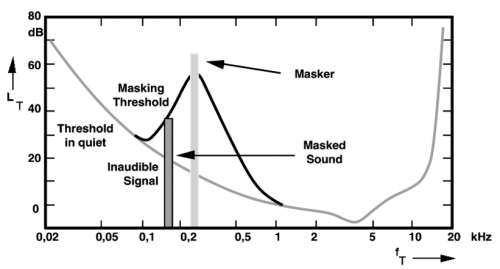
\includegraphics[scale=0.7]{masking_threshold.png}
			\caption{Soglia di mascheramento.}
			\label{fig:masking_threshold}
		\end{figure}
		
		\begin{figure}[h!]
			\centering
				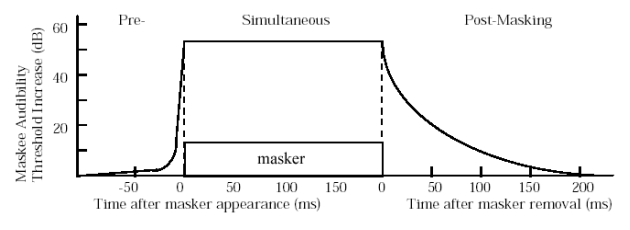
\includegraphics[scale=1]{time_mask.png}
			\caption{Mascheramento temporale.}
			\label{fig:time_mask}
		\end{figure}
		
		L'effetto di mascheramento può essere visto come un'imperfezione dell'orecchio umano, tuttavia rappresenta il punto di forza dell'MP3 e della codifica percettiva: se in un certo lasso di tempo alcune parti del suono vengono percepite con più difficoltà rispetto ad altre, allora possiamo pensare di assegnare più bit per l'informazione del suono predominante e meno per le parti nascoste dal mascheramento. In questo modo l'errore (o distorsione) relativo alle parti mascherate verrà comunque percepito poco, senza degradare più di tanto la qualità complessiva.
		
		
	\chapter{Struttura di un file \texttt{.mp3}} \label{chap:struttura_file_mp3}
	
	\mylettrine{P}{rima} di andare ad analizzare come funziona la codifica (e decodifica) MP3, studiamo com'è fatto un file \texttt{.mp3}, ovvero cosa ci si aspetta di ottenere dalla codifica.\\
	\\
	Un file \texttt{.mp3} è suddiviso in parti dette \textit{frame}. Ogni frame contiene 1152 campioni e dura circa 26 \textit{ms}, il che significa che verranno riprodotte circa 38 \textit{fps} (\textit{frame per secondo}). Inoltre, ogni frame è suddiviso in due \textit{granuli} di 576 sample l'uno.\\
	La dimensione in \textit{byte} di ogni frame dipende sia dal bit rate che dalla sampling frequency scelti, secondo la seguente formula:
	
	\begin{equation} \label{eqn:dimensione_frame}
		\mbox{dimensione frame}=\frac{144\cdot\mbox{bitRate}}{\mbox{samplingRate}}+\mbox{padding}.
	\end{equation}
	
	Il bit di \textit{padding} (allocato all'inizio di ogni frame) è utilizzato per rispettare l'esatto bitrate per tutti i frame (dato che dividendo il bitrate per il numero di frame per secondo si potrebbe non ottenere un intero). Se è impostato ad uno allora la dimensione del frame corrispondente viene aumentata di un byte.\\
	Si tenga ben presente che la dimensione di ogni frame dev'essere sempre un intero, in caso contrario si effettuerà un arrotondamento.
	
	\section{Struttura dei frame} \label{sec:struttura_frame}
		
		La struttura generale di ogni frame è mostrata in Figura \ref{fig:frame_layout}.
		
		\begin{figure}[h!]
			\centering
				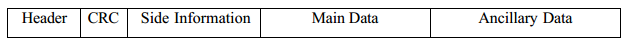
\includegraphics[scale=1]{frame_layout.png}
			\caption{Struttura di un frame.}
			\label{fig:frame_layout}
		\end{figure}
		
		Come possiamo vedere, ogni frame è suddiviso in:
		
		\begin{itemize}
			\item \textit{Header}: detto anche \textit{Intestazione}, è la parte iniziale di ogni frame;
			\item \textit{CRC}: \textit{Cyclic Redundancy Check}, controlla che non ci siano errori nel frame;
			\item \textit{Side Information}: informazione necessaria per decodificare la parte audio del frame;
			\item \textit{Main Data}: gli effettivi dati audio da decodificare;
			\item \textit{Ancillary Data}: detto anche \textit{Dati Ausiliari}, sono dati opzionali destinati a funzioni accessorie.
		\end{itemize}
		
		\subsection{Header} \label{subsec:header}
		
			L'header del frame MP3 ha una lunghezza fissa di 32 bit. La Figura \ref{fig:header_layout} mostra la struttura di un generico frame header.\\
			
			\begin{figure}[h!]
				\centering
					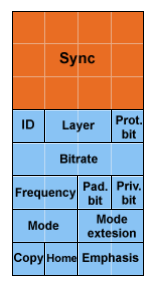
\includegraphics[scale=1.5]{header_layout.png}
				\caption{Struttura dell'header del frame.}
				\label{fig:header_layout}
			\end{figure}
		
		Analizziamo di seguito i vari campi che compongono l'header:
		\begin{itemize}
			\item \textit{Sync} (12 bit): questi bit di sincronizzazione sono sempre impostati tutti a 1 e servono a determinare dove inizia un nuovo frame.
			
			\item \textit{ID} (1 bit): specifica la versione MPEG. Se il bit è asserito significa che il frame è stato codificato con MPEG-1, altrimenti con MPEG-2. Alcuni encoder MP3, inoltre, allocano soltanto 11 bit per la parte Sync per poterne utilizzare 2 per l'ID, secondo la Tabella \ref{tab:campo_id}.
			
				\begin{table}[h!]
					\centering
					\begin{tabular}{|c|c|}
						\multicolumn{1}{c}{\textbf{bit}} & \multicolumn{1}{c}{\textbf{Versione MPEG}}\\
						\hline
						00 & MPEG-2.5 (aggiornamento dell'MPEG-2)\\
						\hline
						01 & Riservato\\
						\hline
						10 & MPEG-2\\
						\hline
						11 & MPEG-1\\
						\hline
					\end{tabular}
					\caption{Valori del campo ID a 2 bit.}
					\label{tab:campo_id}
				\end{table}
				
			\item \textit{Layer} (2 bit): come per il campo ID, i 2 bit del campo Layer indicano quale Layer dello standard MPEG si sta utilizzando, secondo la Tabella \ref{tab:campo_layer}.
			
				\begin{table}[h!]
					\centering
					\begin{tabular}{|c|c|}
						\multicolumn{1}{c}{\textbf{bit}} & \multicolumn{1}{c}{\textbf{Layer MPEG}}\\
						\hline
						00 & Riservato\\
						\hline
						01 & Layer III\\
						\hline
						10 & Layer II\\
						\hline
						11 & Layer I\\
						\hline
					\end{tabular}
					\caption{Valori del campo Layer.}
					\label{tab:campo_layer}
				\end{table}
			
			\item \textit{Protection bit} (1 bit): se asserito, allora viene utilizzato il campo CRC per la rilevazione di errori nel frame.
			
			\item \textit{Bitrate} (4 bit): questi quattro bit, assieme ai campi ID e Layer, informano il decoder sul bitrate richiesto, secondo la Tabella \ref{tab:campo_bitrate}. Ovviamente se il file \texttt{.mp3} è codificato con CBR (Constant BitRate), allora tutti i frame avranno lo stesso valore nel campo Bitrate.
			
				\begin{table}[h!]
					\centering
					\begin{tabular}{c|c|c|c|c|c|c|}
						\multirow{2}{*}{\textbf{bit}} & \multicolumn{3}{|c|}{\textbf{MPEG-1}} & \multicolumn{3}{|c|}{\textbf{MPEG-2}}\\
						\cline{2-7}
						& \textbf{Layer I} & \textbf{Layer II} & \textbf{Layer III} & \textbf{Layer I} & \textbf{Layer II} & \textbf{Layer III}\\
						\hline
						0000 & & & & & &\\
						\hline
						0001 & 32 & 32 & 32 & 32 & 32 & 8\\
						\hline
						0010 & 64 & 48 & 40 & 64 & 48 & 16\\
						\hline
						0011 & 96 & 56 & 48 & 96 & 56 & 24\\
						\hline
						0100 & 128 & 64 & 56 & 128 & 64 & 32\\
						\hline
						0101 & 169 & 80 & 64 & 160 & 80 & 64\\
						\hline
						0110 & 192 & 96 & 80 & 192 & 96 & 80\\
						\hline
						0111 & 224 & 112 & 96 & 224 & 112 & 56\\
						\hline
						
						1000 & 256 & 128 & 112 & 256 & 128 & 64\\
						\hline
						1001 & 288 & 160 & {\color{red} 128} & 288 & 160 & {\color{red} 128}\\
						\hline
						1010 & 320 & 192 & 160 & 320 & 192 & 160\\
						\hline
						1011 & 352 & 224 & 192 & 352 & 224 & 112\\
						\hline
						1100 & 384 & 256 & 224 & 384 & 256 & 128\\
						\hline
						1101 & 416 & 320 & 256 & 416 & 320 & 256\\
						\hline
						1110 & 448 & 384 & 320 & 448 & 384 & 320\\
						\hline
						1111 & & & & & &\\
						\hline
						
					\end{tabular}
					\caption[Valori del campo Bitrate.]{Valori del campo Bitrate (i valori in rosso rappresentano la scelta più frequente).}
					\label{tab:campo_bitrate}
				\end{table}
			
			\item \textit{Frequency} (2 bit): questi 2 bit indicano la sampling frequency utilizzata, come indicato in Tabella \ref{tab:campo_frequency}.
			
				\begin{table}[h!]
					\centering
					\begin{tabular}{|c|c|c|c|}
						\multicolumn{1}{c}{\textbf{bit}} & \multicolumn{1}{c}{\textbf{MPEG-1}} & \multicolumn{1}{c}{\textbf{MPEG-2}} & \multicolumn{1}{c}{\textbf{MPEG-2.5}}\\
						\hline
						00 & 44.1 \textit{kHz} & 22.05 \textit{kHz} & 11.025 \textit{kHz}\\
						\hline
						01 & 48 \textit{kHz} & 24 \textit{kHz} & 12 \textit{kHz}\\
						\hline
						10 & 32 \textit{kHz} & 16 \textit{kHz} & 8 \textit{kHz}\\
						\hline
						11 & \multicolumn{3}{|c|}{Riservato}\\
						\hline
					\end{tabular}
					\caption{Valori del campo Frequency.}
					\label{tab:campo_frequency}
				\end{table}
			
			\item \textit{Padding bit} (1 bit): come già accennato riguardo alla dimensione dei frame, se con la (\ref{eqn:dimensione_frame}) si ottiene un numero decimale, per alcuni frame si arritonderà per eccesso, mentre per altri per difetto. Se ad esempio si utilizza un bitrate di 128 \textit{bps} ed una sampling frequency di 44.1 \textit{kHz}, si avrà la dimensione dei frame pari a circa 417.95 byte, ovvero si avranno frame da 417 e frame da 418, per rispettare il bitrate indicato. Se il bit di padding è settato, allora il frame attuale è stato arrotondato per eccesso.
			
			\item \textit{Private bit} (1 bit): bit a uso specifico delle applicazioni.
			
			\item \textit{Mode} (2 bit): riprendendo quanto detto riguardo alle modalità di canale, i bit Mode indicheranno la modalità del frame attuale secondo la Tabella \ref{tab:campo_mode}.
			
				\begin{table}[h!]
					\centering
					\begin{tabular}{|c|c|}
						\multicolumn{1}{c}{\textbf{bit}} & \multicolumn{1}{c}{\textbf{Channel Mode}}\\
						\hline
						00 & Stereo\\
						\hline
						01 & Joint Stereo\\
						\hline
						10 & Canale Doppio\\
						\hline
						11 & Canale Singolo\\
						\hline
					\end{tabular}
					\caption{Valori del campo Mode.}
					\label{tab:campo_mode}
				\end{table}
			
			\item \textit{Mode Extension} (2 bit): bit utilizzati soltanto nel caso in cui la modalità di canale sia impostata su joint stereo, nel qual caso il campo Mode Extension indicherà se viene utilizzata la tecnica MS stereo, intensity stereo o una combinazione delle due (si veda la Tabella \ref{tab:campo_mode_extension}).
			
				\begin{table}[h!]
					\centering
					\begin{tabular}{|c|c|c|}
						\multicolumn{1}{c}{\textbf{bit}} & \multicolumn{1}{c}{\textbf{MS stereo}} & \multicolumn{1}{c}{\textbf{Intensity stereo}}\\
						\hline
						00 & off & off\\
						\hline
						01 & off & on\\
						\hline
						10 & on & off\\
						\hline
						11 & on & on\\
						\hline
					\end{tabular}
					\caption{Valori del campo Mode Extension.}
					\label{tab:campo_mode_extension}
				\end{table}
			
			\item \textit{Copy} (1 bit): se questo bit è asserito, allora significa che il contenuto è coperto da copyright ed è illegale copiarlo.
			
			\item \textit{Home} (1 bit): se asserito, indica che il frame si trova nel file originale.
			
			\item \textit{Emphasis} (2 bit): bit di enfasi che indicano come ri-equalizzare il suono dopo un'eliminazione del rumore di tipo Dolby (raramente usati). Per conoscenza, si veda la Tabella \ref{tab:campo_emphasis}.
			
				\begin{table}[h!]
					\centering
					\begin{tabular}{|c|c|}
						\multicolumn{1}{c}{\textbf{bit}} & \multicolumn{1}{c}{\textbf{Modello di soppressione del rumore}}\\
						\hline
						00 & Nessuno\\
						\hline
						01 & 50/15 \textit{ms}\\
						\hline
						10 & Riservato\\
						\hline
						11 & CCITT J.17\\
						\hline
					\end{tabular}
					\caption{Valori del campo Emphasis.}
					\label{tab:campo_emphasis}
				\end{table}
			
		\end{itemize}
		
		\subsection{CRC} \label{subsec:crc}
			
			Il campo CRC (di 0 o 16 bit) è una Cyclic Redundancy Check sui dati sensibili del frame, per evitare che contengano errori. Se il bit Protection nell'header è asserito, allora il campo CRC conterrà una checksum dei bit dal 16 al 32 dell'header e della side information (che secondo lo standard contengono i dati più sensibili del frame). Se un frame risulta danneggiato, può essere mutato o rimpiazzato dal frame precedente.
		
		\subsection{Side Information} \label{subsec:side_information}
			
			Il campo Side Information contiene tutte quelle informazioni necessarie al decoder per decodificare i dati audio di ogni frame. Se si utilizza un canale singolo, allora questo campo sarà lungo 17 byte, altrimenti 32. La struttura del campo Side Information è mostrato in Figura \ref{fig:side_information_layout}.\\
			
			\begin{figure}[h!]
				\centering
					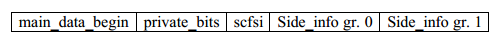
\includegraphics[scale=1.2]{side_information_layout.png}
				\caption{Struttura del campo Side Information.}
				\label{fig:side_information_layout}
			\end{figure}
		
			Analizziamo di seguito i campi della Side Information. Dal momento che le dimensioni dei vari campi possono variare a seconda della modalità di canale scelta, tra parentesi verranno indicate le dimensioni per la modalità mono (primo valore) e le dimensioni per tutte le altre modalità (secondo valore). Se invece è indicato un solo valore, la dimensione di quel campo è costante. Inoltre, tutte le tabelle si riferiscono alla modalità mono.
			
			\begin{itemize}
				\item \textit{main\_data\_begin} (9 bit): utilizzando il formato del Layer III, viene impiegata una tecnica detta \textit{bit reservoir} (letteralmente, \textit{deposito di bit}), che consente di sfruttare lo spazio inutilizzato nel campo Main Data di un frame da frame consecutivi. Il campo main\_data\_begin è un numero negativo che indica quanti byte prima (rispetto al primo bit della synchronization word) iniziano i dati principali, escludendo dal conteggio le parti statiche di un frame, come l'header. Essendo un campo a 9 bit, i dati principali possono iniziare fino a $(2^9-1) \cdot 8 = 4088$ bit prima, che corrisponde a svariati frame. Se il campo è impostato a 0, allora i dati principali iniziano subito dopo la Side Information.
				
				\item \textit{private\_bits} (5 bit, 3 bit): bit privati destinati all'utilizzo specifico da parte delle applicazioni.
				
				\item \textit{scfsi} (4 bit, 8 bit): la \textit{ScaleFactor Selection Information} (o \textit{Informazione sulla Selezione dei Fattori di Scala}) indica se dei certi \textit{scalefactor} (\textit{fattori di scala}, vedremo più avanti cosa sono) sono condivisi oppure no tra i due granuli di un frame. Le bande di fattori di scala sono suddivise in 4 gruppi, secondo la Tabella \ref{tab:gruppi_scalefactor}. In questo campo, vengono trasmessi 4 bit per ogni canale: se il bit del gruppo è asserito, allora quelle scalefactor band valgono sia per il granulo 0 che per il granulo 1, così da poterle trasmettere una sola volta.
				
					\begin{table}[h!]
						\centering
						\begin{tabular}{|c|c|}
							\multicolumn{1}{c}{\textbf{Gruppo}} & \multicolumn{1}{c}{\textbf{Scalefactor Band}}\\
							\hline
							0 & 0, 1, 2, 3, 4, 5\\
							\hline
							1 & 6, 7, 8, 9, 10\\
							\hline
							2 & 11, 12, 13, 14, 15\\
							\hline
							3 & 16, 17, 18, 19, 20\\
							\hline
						\end{tabular}
						\caption{Gruppi delle scalefactor band}
						\label{tab:gruppi_scalefactor}
					\end{table}
				
				\item \textit{Side\_info}: le ultime due parti della Side Information (``Side\_info gr.0'' e ``Side\_info gr.1'') contengono le informazioni per la decodifica dei due granuli del frame e sono strutturalmente identiche (si veda la Figura \ref{fig:side_info_gr_layout}).
				
					\begin{figure}[h!]
						\centering
							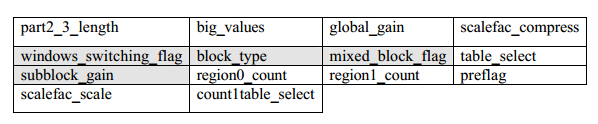
\includegraphics[scale=1]{side_info_gr_layout.png}
						\caption{Struttura della Side Information per ogni granulo.}
						\label{fig:side_info_gr_layout}
					\end{figure}
					
					Di seguito, l'analisi dei sottocampi che compongono la Side Information di ogni granulo:
					
					\begin{itemize}
						
						\item \textit{part2\_3\_length} (12 bit, 24 bit): indica quanti bit allocare nel campo Main Data per i fattori i scala (part2) e per i dati codificati con Huffman (part3) (più avanti vedremo com'è composto il campo Main Data).
						
						\item \textit{big\_values} (9 bit, 18 bit): i 576 sample contenuti in ogni granulo non sono necessariamente codificati tutti con la stessa tabella di Huffman. In particolare, le frequenze di questi sample, che spaziano da 0 al limite di Nyquist, verranno suddivise in 5 regioni (Figura \ref{fig:frequency_regions}), ognuna della quali codificata con una diversa tabella di Huffman. L'obiettivo è quello di rendere la codifica di Huffman ancora più efficiente codificando in modo diverso diverse parti dello spettro.
						
							\begin{figure}[h!]
								\centering
									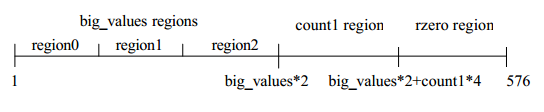
\includegraphics[scale=1]{frequency_regions.png}
								\caption{Regioni di frequenza.}
								\label{fig:frequency_regions}
							\end{figure}
							
							Nella regione rzero si trovano le frequenze più alte, divise a coppie. Nella regione count1 si trovano frequenze più basse di quelle in rzero, suddivise in gruppi di quattro. Infine, nelle regioni big values si trovano tutte le altre frequenze che arrivano fino a zero. Il massimo valore assoluto di ampiezza per i sample nelle regioni big values è limitato a 8191. Dal momento che il campo big\_values determina la grandezza delle regioni big values, il massimo valore possibile per questo campo è 288 \footnote{Calcolato come $576/2$, in quanto la dimensione della regione di big values è calcolata come $big\_values\cdot 2$.}.
						
						\item \textit{global\_gain} (8 bit, 16 bit): specifica la grandezza dello step di quantizzazione.
						
						\item \textit{scalefac\_compress} (4 bit, 8 bit): determina il numero di bit utilizzati per i fattori di scala. Ogni granulo può essere diviso in 12 (per finestre corte) o 21 (per finestre lunghe) bande di fattori di scala. Non spiegheremo qui cosa si intende con finestre, in quanto verrà spiegato più ampiamente all'interno del Capitolo \ref{chap:codifica}. Le bande di fattori di scala sono successivamente suddivise in due parti (0-6, 7-11 per finestre corte e 0-10, 11-20 per finestre lunghe), rispettivamente lunghe \textit{slen1} e \textit{slen2}. A seconda del valore del campo scalefac\_compress, verranno assegnati più o meno bit alle due parti, come mostrato in Tabella \ref{tab:campo_scalefac_compress}.
						
							\begin{table}[h!]
								\centering
								\begin{tabular}{|c|c|c|}
									\multicolumn{1}{c}{\textbf{bit}} & \multicolumn{1}{c}{\textbf{slen1}} & \multicolumn{1}{c}{\textbf{slen2}}\\
									\hline
									0000 & 0 & 0\\
									\hline
									0001 & 0 & 1\\
									\hline
									0010 & 0 & 2\\
									\hline
									0011 & 0 & 3\\
									\hline
									0100 & 3 & 0\\
									\hline
									0101 & 1 & 1\\
									\hline
									0110 & 1 & 2\\
									\hline
									0111 & 1 & 3\\
									\hline
									1000 & 2 & 1\\
									\hline
									1001 & 2 & 2\\
									\hline
									1010 & 2 & 3\\
									\hline
									1011 & 3 & 1\\
									\hline
									1100 & 3 & 2\\
									\hline
									1101 & 3 & 3\\
									\hline
									1110 & 4 & 2\\
									\hline
									1111 & 4 & 3\\
									\hline
								\end{tabular}
								\caption{Valori del campo scalefac\_compress.}
								\label{tab:campo_scalefac_compress}
							\end{table}
						
						\item \textit{windows\_switching\_flag} (1 bit, 2 bit): se asserito, indica che sarà utilizzata una finestra diversa da quella di default (si veda Capitolo \ref{chap:codifica}). Inoltre quando è asserito, tutti i valori (big values) che non sono contenuti nella region0 sono contenuti nella region1, rendendo la region2 di fatto vuota.
						
						\item \textit{block\_type} (2 bit, 4 bit): se il bit windows\_switching\_flag è asserito, allora questo campo serve a indicare il tipo di finestra utilizzato per il granulo corrente. I valori 1 e 3 sono finestre lunghe, mentre il valore 2 indica una finestra corta. Il valore 0 indicherebbe la finestra normale di default (lunga), ma dato che quando si usa la finestra di default il campo block\_type non viene utilizzato, questo valore è vietato. Vediamo nel dettaglio il significato di questi valori in Tabella \ref{tab:campo_block_type} (per i vari tipi di finestra si rimanda sempre al Capitolo \ref{chap:codifica}).
						
							\begin{table}[h!]
								\centering
								\begin{tabular}{|c|c|}
									\multicolumn{1}{c}{\textbf{bit}} & \multicolumn{1}{c}{\textbf{Tipo finestra}}\\
									\hline
									00 & Vietato\\
									\hline
									01 & Finestra inizio\\
									\hline
									10 & 3 finestre corte\\
									\hline
									11 & Finestra fine\\
									\hline
								\end{tabular}
								\caption{Valori del campo block\_type.}
								\label{tab:campo_block_type}
							\end{table}
						
						\item \textit{mixed\_block\_flag} (1 bit, 2 bit): se asserito, indica che le due sottobande più basse (si veda il Capitolo \ref{chap:codifica} per quanto riguarda le sottobande) sono trasformate utilizzando la finestra normale, mentre le restanti 30 utilizzando la finestra indicata dal campo block\_type. Questo campo viene utilizzato soltanto se il bit windows\_switching\_flag è asserito.
						
						\item \textit{table\_select} (10 bit, 20 bit) o (15 bit, 30 bit): lo standard MP3 definisce 32 possibili tabelle di Huffman con cui codificare i sample. Essendo le tabelle possibili 32, servono 5 bit (per canale, granulo e regione) per individuare univocamente una tabella. Il campo table\_select definisce con quali tabelle di Huffman decodificare i sample delle regioni big values. Quindi se windows\_switching\_flag è settato a 1 la regione region2 sarà vuota e si avranno 10 bit (in modalità mono) necessari per l'individuazione delle tabelle di Huffman (20 se in modalità stereo). Se invece il bit è negato si avrà bisogno di altri 5 bit per canale per la tabella relativa alla regione region2, ovvero 15 bit per mono e 30 per stereo.
						
						\item \textit{subblock\_gain} (9 bit, 18 bit): se windows\_switching\_flag=1 e block\_type=10, allora questo campo definisce, 3 bit alla volta, l'offset da aggiungere al global\_gain per ogni sottoblocco.
										
						\item \textit{region0\_count}(4 bit, 8 bit): in questo campo viene indicato il numero di bande di fattori di scala presenti nella regione region0 diminuito di 1. Quindi se ad esempio region0\_count=8, allora nella regione region0 ci sono 9 bande di fattori di scala. Inoltre se utilizzano finestre corte (block\_type=10), allora in questo campo vengono contate le bande dei fattori di scala per ogni sottoblocco: se, ad esempio, in questo caso avessimo sempre region0\_count=8, allora nella regione region0 ci sarebbero 9/3=3 bande di fattori di scala. Questo campo viene utilizzato per ricavare gli estremi della regione region0, infatti questi estremi vengono allineati (nella partizione dello spettro in regioni) per combaciare con la suddivisione delle frequenze in bande di fattori di scala.
						
						\item \textit{region1\_count}(3 bit, 6 bit): esattamente come il campo region0\_count, solo rispetto alla regione region1.
						
						\item \textit{preflag}(1 bit, 2 bit): è un bit che permette l'amplificazione di alte frequenze quantizzate. Se asserito, i valori di una tabella predefinita vengono sommati alle bande di fattori di scala. Se si usano finestre corte (block\_type=10) questo campo non si usa mai.
						
						\item \textit{scalefac\_scale}(1 bit, 2 bit): i fattori di scala sono quantizzati logaritmicamente con uno step di quantizzazione pari a 2 o $\sqrt{2}$, secondo la Tabella \ref{tab:campo_scalefac_scale}.
						
							\begin{table}[h!]
								\centering
								\begin{tabular}{|c|c|}
									\multicolumn{1}{c}{\textbf{bit}} & \multicolumn{1}{c}{\textbf{Dimensione step}}\\
									\hline
									0 & $\sqrt{2}$\\
									\hline
									1 & 2\\
									\hline
								\end{tabular}
								\caption{Valori del campo scalefac\_scale.}
								\label{tab:campo_scalefac_scale}
							\end{table}
						
						\item \textit{count1table\_select} (1 bit, 2 bit): questo bit seleziona una delle due possibili tabelle di Huffman per la decodifica della regione count1.
						
					\end{itemize}
				
			\end{itemize}
		
		\subsection{Main Data} \label{subsec:main_data}
			
			La parte di dati principali consiste nei fattori di scala e nei sample quantizzati codificati con Huffman. Lo schema in Figura \ref{fig:main_data_layout} rappresenta la struttura del campo Main Data.
			
			\begin{figure}[h!]
				\centering
					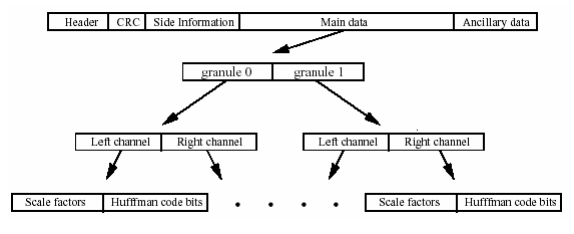
\includegraphics[scale=1]{main_data_layout.png}
				\caption{Struttura del campo Main Data in modalità stereo.}
				\label{fig:main_data_layout}
			\end{figure}
			
			\begin{itemize}
				\item \textit{Fattori di scala}: i \textit{fattori di scala} (o \textit{scalefactor}) vengono utilizzati per ridurre il rumore da quantizzazione e rappresentano delle approssimazioni delle bande critiche dell'orecchio umano (che sono 24). Se scelti correttamente in fase di codifica, la maggior parte del rumore di quantizzazione sparirà, per effetto del mascheramento. Per ogni banda di fattori di scala, viene trasmesso (scelto) un solo fattore di scala. Il campo scfsi determina se (e quali) fattori di scala sono condivisi dai due granuli, in modo da trasmetterli una sola volta. I bit effettivi allocati per i fattori di scala dipendono dal valore del campo scalefac\_compress.\\
					La suddivisione delle frequenze dello spettro in bande di fattori di scala è fissata a seconda del tipo di finestra e della sampling frequency. La suddivisione effettiva è memorizzata in tabelle all'interno dell'encoder e del decoder MP3.
				
				\item \textit{Codifica Huffman}: questa parte dei dati principali contiene i valori codificati tramite codifica di Huffman. Le informazioni su come decodificare questi dati sono contenute nel campo Side Information. Ricordiamo che i valori delle regioni big values sono codificati a coppie, mentre quelli della regione count1 sono codificati a gruppi di 4.
				
			\end{itemize}
		
		\subsection{Ancillary Data} \label{subsec:ancillary_data}
			
			La parte di dati aggiuntivi è opzionale e la sua lunghezza è variabile e non esplicitata. Inizia subito dopo la codifica Huffman del secondo granulo ed arriva fino alla word di sincronizzazione del frame successivo. Questi dati possono essere usati per scopi specifici all'interno di determinate applicazioni.
		
	\section{ID3} \label{sec:id3}
		
		Anche se l'MP3 riesce ad ottenere una notevole compressione audio senza un'eccessiva perdita di qualità, esso manca della possibilità di aggiungere informazioni testuali. Infatti, specialmente per quando riguarda le canzoni, risulta molto comodo salvare all'interno del file \texttt{.mp3}  informazioni testuali come autore o titolo della canzone.\\
		Per soddisfare queste esigenze nacque il cosiddetto ID3, ovvero una serie di tag (di 128 byte) memorizzati alla fine del file \texttt{.mp3}. I tag disponibili erano i seguenti:
		
		\begin{itemize}
			\item titolo (30 byte);
			\item artista (30 byte);
			\item album (30 byte);
			\item anno (4 byte);
			\item commento (30 byte);
			\item genere (1 byte).
		\end{itemize}
		
		Inoltre un file \texttt{.mp3} che volesse fare uso dei tag ID3 doveva scrivere subito dopo i dati aggiuntivi la parola ``TAG'', per indicare dove iniziavano i tag ID3. Escludendo la parola ``TAG'', la somma dei tag ID3 misurava sempre 128 byte (lo spazio inutilizzato veniva riempito con zeri).\\
		\\
		In una variante dell'ID3, detta ID3 v1.1 (Figura \ref{fig:id3v1_1_layout}) al tag del commento sono stati sottratti due bit per aggiungere un tag \textit{traccia} (riferendosi al numero di traccia della canzone nel CD di provenienza) di 1 byte ed un byte nullo tra il commento ed il numero di traccia.\\
		
		\begin{figure}[h!]
			\centering
				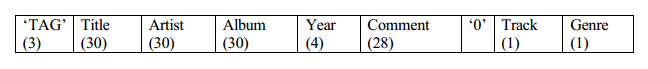
\includegraphics[scale=1]{id3v1_1_layout.png}
			\caption{Struttura dei tag ID3 v1.1.}
			\label{fig:id3v1_1_layout}
		\end{figure}
		
		Le prime versioni di ID3, tuttavia, avevano diversi aspetti negativi, come il fatto di avere pochi campi e che questi avessero una lunghezza massima di 30 byte. Inoltre, dato che le informazioni erano memorizzate alla fine del file \texttt{.mp3} non era possibile ottenerle durante uno streaming in tempo reale. Venne quindi rilasciata una versione più complessa, detta ID3 v2, che memorizzava i tag all'inizio del file \texttt{.mp3}, metteva a disposizione più campi e non imponeva un limite massimo di byte, in quanto supportava dimensioni dinamiche. Attualmente (\monthyear\today) l'ultima versione rilasciata dell'ID3 è l'ID3 v2.4.
	\chapter{Codifica} \label{chap:codifica}
	
	Iniziamo finalmente l'analisi dell'algoritmo di compressione MP3. I passi principali di quest'algoritmo sono illustrati in Figura \ref{fig:encode_layout}.\\
	
	\begin{figure}[h!]
		\centering
			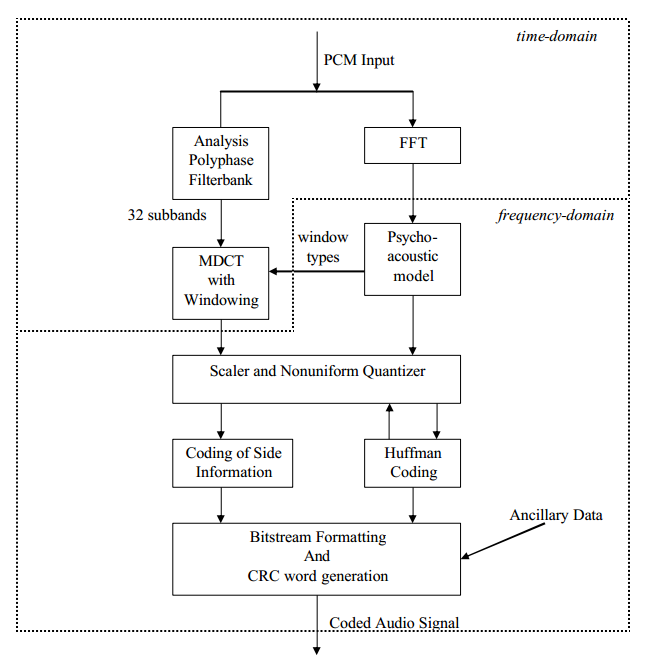
\includegraphics[scale=0.8]{encode_layout.png}
		\caption{Schema della codifica MP3.}
		\label{fig:encode_layout}
	\end{figure}
	
	Di seguito verranno illustrate le varie fasi, senza tuttavia entrare troppo nel dettaglio o in ambito implementativo.
	
	\section{Banco filtri ibrido}
		
		Il primo passo della codifica MP3 consiste nel suddividere i sample PCM in sottobande e nel mapparli in sample a dominio di frequenza. Questo procedimento, detto \textit{banco filtri ibrido}, è composto da un \textit{banco filtri di analisi polifasico} e dall'algoritmo \textit{MDCT}.
		
		\subsection{Banco filtri di analisi polifasico} \label{subsec:banco_filtri_analisi_polifasico}
			
			La prima fase consiste in un banco di filtri di analisi polifasico, che prende in input 1152 sample PCM e restituisce come output 1152 sample divisi in 32 sottobande equispaziate, ovvero suddivide il segnale di input nelle sue componenti raggruppate per sottobanda. Gli estremi delle 32 sottobande sono definiti dalla sampling frequency utilizzata per ottenere i campioni PCM e dal limite di Nyquist corrispondente: se ad esempio la frequenza di campionamento è 44.1 \textit{kHz}, le frequenze campionate vanno da 0 a 22.05 \textit{kHz}, quindi ogni sottobanda sarà larga $22050/32\approx 689$ \textit{Hz}. Le sottobande saranno in questo caso 0-689 \textit{Hz}, 689-1378 \textit{Hz}, 1378-2067 \textit{Hz}, ecc\dots.
			
			\begin{wrapfigure}{r}{0.5\textwidth}
				\centering
					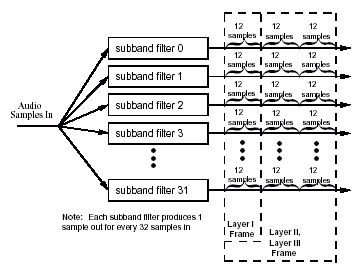
\includegraphics[scale=1]{filterbank.png}
				\caption{Banco filtri di analisi polifasico.}
				\label{fig:filterbank}
			\end{wrapfigure}
			
			Dal momento che, virtualmente, ogni sample PCM può contenere componenti di ogni sottobanda, il banco di filtri di analisi produce, di fatto, 32 sample (uno per ogni sottobanda) per ogni sample PCM, aumentando il numero di sample di un fattore 32. Quindi viene eseguito un \textit{downsampling} (o \textit{decimazione}) di fattore 32 (ovvero si prende un sample ogni 32), in modo da avere nuovamente 1152 sample. Ovviamente, il downsampling inserisce dell'aliasing (è quindi un procedimento lossy).\\
			Il banco filtri di analisi polifasico è costruito mettendo in parallelo 32 filtri passa-banda, ognuno destinato a far passare soltanto le frequenze appartenenti alla sottobanda corrispondente. Ogni sottobanda sarà composta da 36 (=1152/32) sample, suddivisi in 3 gruppi da 12, come mostrato in Figura \ref{fig:filterbank}.
		
		\subsection{MDCT} \label{subsec:MDCT}
		
			Applicando una \textit{Trasformata Discreta del Coseno Modificata} (\textit{MDCT}, \textit{Modified Discrete Cosine Transform}) ognuna delle 32 sottobande viene suddivida in 18 sottobande più fini, andando a formare un granulo di 576 linee di frequenza (anche se di fatto sono bande di frequenza, l'ampiezza di banda è talmente fine che vengono spesso chiamate linee di frequenza). Inoltre, essendo un tipo particolare di Trasformata Discreta del Coseno, e quindi della Trasformata di Fourier, i sample in input a dominio di tempo vengono trasformati in coefficienti a dominio di frequenza.\\
			L'MDCT prende in input i 1152 sample generati dal banco filtri di analisi polifasico (corrispondenti ad un frame, o due granuli) e produce in output 576 ($=32\cdot 18$) linee di frequenza (corrispondenti a un granulo). La MDCT si basa sulla sovrapposizione degli input (a due a due) per produrre gli output, secondo lo schema in Figura \ref{fig:mdct}.\\
			
			\begin{figure}[h!]
				\centering
					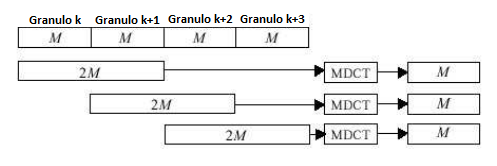
\includegraphics[scale=1]{mdct.png}
				\caption{Trasformazione MDCT.}
				\label{fig:mdct}
			\end{figure}
			
			In generale, la MDCT prende in input $2N$ sample $\{y_n\}$, $n=0,\dots,2N-1$, e restituisce in output $N$ sample a dominio di frequenza $\{x_k\}$, $k=0,\dots,N-1$, secondo la seguente formula:
			
			\begin{equation} \label{eqn:mdct}
				x_k = \sum_{n=0}^{2N-1}y_n\cdot\cos\left[\frac{\pi}{N}\left(n+\frac{1}{2}+\frac{N}{2}\right)\left(k+\frac{1}{2}\right)\right], \qquad k=0,\dots,N-1.
			\end{equation}
			
			Prima di applicare la MDCT è tuttavia necessario utilizzare una funzione di finestra per eliminare (assieme alla MDCT) gli artefatti temporali durante una transizione di frame. Lo standard MP3 definisce quattro tipi di finestre (Figura \ref{fig:windows}), a seconda della stazionarietà del modello psicoacustico.\\
			
			\begin{figure}[h!]
				\centering
					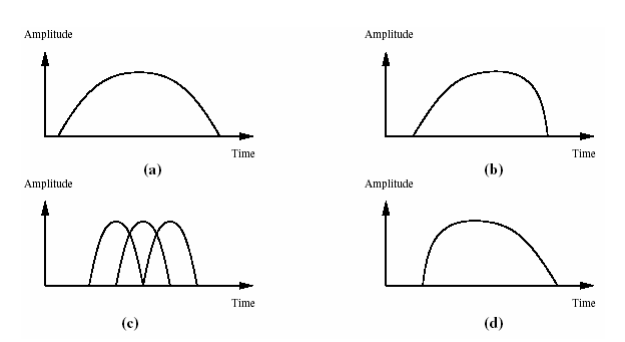
\includegraphics[scale=1]{windows.png}
				\caption[Tipologie di finestre.]{Tipologie di finestre: (a) finestra lunga; (b) finestra inizio; (c) 3 finestre corte; (d) finestra fine.}
				\label{fig:windows}
			\end{figure}
			
			Se il modello psicoacustico decide che (per ogni sottobanda) il segnale non cambia, o cambia poco, tra il frame corente e quello precedente, allora viene utilizzata una \textit{finestra lunga}, che migliora la risoluzione spettrale (ovvero sulla frequenza) data dall'MDCT. Se al contrario vi sono notevoli differenze, allora vengono utilizzate \textit{tre finestre corte} (sovrapposte) per migliorare la risoluzione temporale data dall'MDCT e quindi eliminare gli artefatti temporali.\\
			Quando si passa da una finestra lunga a finestre corte, si utilizza una \textit{finestra inizio}. Viceversa, se si passa da finestre corte ad una finestra lunga si utilizza una \textit{finestra fine}.\\
			In concreto, l'applicazione della funzione finestra consiste nel moltiplicare ogni input per una funzione seno (a seconda della finestra utilizzata).\\
			\\
			Come già accennato, la decimazione fatta dal banco di filtri di analisi polifasico introduce dell'aliasing, ma permette di inviare meno informazioni. L'aliasing in questione verrà ridotto in fase di decodifica tramite calcoli ``a farfalla'', come vedremo nel Capitolo \ref{chap:decodifica}.
			
	\section{Fast Fourier Transform} \label{sec:fft}
		
		Dal momento che la risoluzione di frequenza data dal banco filtri è troppo bassa, simultaneamente al banco filtri di analisi polifasico viene effettuata una \textit{Trasformata di Fourier veloce}, o \textit{Fast Fourier Transform} (\textit{FFT}), in modo da avere una miglior risoluzione e più informazioni sul cambiamento di frequenza nel tempo. La FFT (che non è altro che una versione ottimizzata della Trasformata Discreta di Fourier) mappa il segnale in entrata a dominio di tempo in un segnale a dominio di frequenza. In questo caso viene utilizzata una FFT a 1024 o 256 punti su 1152 sample PCM in entrata.
		
	\section{Modello psicoacustico} \label{sec:modello_psicoacustico}
		
		Questa fase rappresenta il modello psicoacustico. Esso prende in input i sample, a dominio di frequenza, generati dalla FFT e fornisce informazioni all'MDCT su quale finestra utilizzare. Inoltre da anche informazioni alla fase di Quantizzazione Non Uniforme su come quantizzare le diverse linee di frequenza.\\
		\\
		Per decidere quale finestra inviare all'MDCT, vengono comparati gli spettri del frame corrente e del frame precedente. Se non vengono rilevati cambiamenti (\textit{no attack}) allora si utilizza una finestra lunga. Se vengono registrati cambiamenti (\textit{attack}), viene effettuato il passaggio da finestra lunga a finestre corte e quest'ultime verranno utilizzate finché il segnale non si stabilizzerà nuovamente. In Figura \ref{fig:psychoacoustic_model} è rappresentato il diagramma di decisione della finestra da inviare all'MDCT.\\
		
		\begin{figure}[h!]
			\centering
				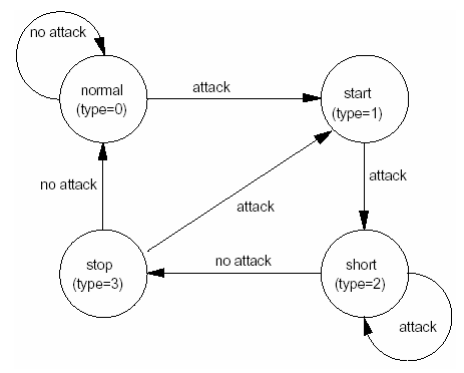
\includegraphics[scale=1]{psychoacoustic_model.png}
			\caption{Modello psicoacustico: diagramma di decisione della finestra.}
			\label{fig:psychoacoustic_model}
		\end{figure}
		
		Il modello psicoacustico, inoltre, analizza lo spettro fornito dalla FFT per indiciduare le componenti dominanti e calcolare la soglia di mascheramento per ogni banda critica (le frequenze sotto questa soglia verranno mascherate). Le soglie di mascheramento di ogni banda critica verranno quindi utilizzate nella Quantizzazione Non Uniforme per diminuire il rumore di quantizzazione.
		
	\section{Quantizzazione Non Uniforme} \label{sec:quantizzazione_non_uniforme}
		
		In questa fase vengono scalati e quantizzati 576 sample a dominio di frequenza per volta. Lo schema generale presenta due cicli annidati: \textit{rate control loop} (ciclo di controllo del tasso, esterno) e \textit{distorsion control loop} (ciclo di controllo della distorsione, interno).
		
		\begin{itemize}
			\item \textit{rate control loop}: in questo ciclo avviene la quantizzazione dei sample. I valori vengono quantizzati più volte, con step di quantizzazione sempre maggiori, fino a che i valori quantizzati non possono essere codificati con una delle tabelle di Huffman disponibili (step di quantizzazione più grandi implicano valori quantizzati più piccoli). Quindi viene calcolata la somma dei bit utilizzati per i valori quantizzati codificati con Huffman: se i bit necessari rientrano nei bit disponibili, allora si passa al loop interno, altrimenti si ripete il processo aumentando lo step di quantizzazione finché i bit disponibili non sono sufficienti. In questo step, inoltre, vengono calcolate anche le regioni e sottoregioni (big values, count1, rzero, ecc\dots) ed i rispettivi limiti. Lo step di quantizzazione viene regolato dal campo global\_gain nella Side Information di ogni granulo (vedi Capitolo \ref{chap:struttura_file_mp3}).
			
			\item \textit{distorsion control loop}: in questo ciclo, invece, viene controllato il rumore di quantizzazione prodotto nel ciclo precedente e vengono quindi aggiustati i fattori di scala finché il rumore non è mascherato per ogni banda di fattori di scala. Si applicano quindi i fattori di scala ad ogni linea di frequenza di ogni banda di fattori di scala, finché tutte le bande di fattori di scala non hanno il rumore inferiore alla soglia di mascheramento calcolata per quella banda (dal modello psicoacustico). Se una banda presenta un rumore di quantizzazione maggiore della soglia di mascheramento, allora il rumore sarà udibile dall'orecchio umano: in questi casi il fattore di scala corrispondente viene aumentato (maggiore è il fattore di scala, meno viene scalato il sample) e il processo ripetuto. Quando finalmente tutte le bande di fattori di scala saranno poco rumorose (ovvero con rumore sotto la soglia di mascheramento) si uscirà dal ciclo di controllo di distorsione, salvando fattori di scala e step di quantizzazione, per entrare nuovamente nel ciclo esterno, in modo da poter utilizzare step di quantizzazione più piccoli (se possibile) con i nuovi valori scalati.
			
		\end{itemize}
		
	\section{Codifica Huffman} \label{sec:codifica_huffman}
		
		Una volta terminata la quantizzazione e la determinazione dei fattori di scala, i valori quantizzati vengono codificati con la tabella di Huffman corrispondente (a seconda delle tabelle scelte per le varie regioni e sottoregioni). Si osservi che, prima della codifica di Huffman, vengono riordinate le linee di frequenza relative alle finestre corte prima per sottobanda, poi per frequenza ed infine per finestra, in quanto sample con frequenza simile hanno più probabilità di avere valori simili (l'output dell'MDCT ordinava questi sample per sottobanda, per finestra e quindi per frequenza).
		
	\section{Strutturazione della Side Information} \label{sec:strutturazione_side_information}
		
		A questo punto tutti i dati generati nelle fasi precedenti (step di quantizzazione, tabelle di huffman, finestre, ecc\dots) vengono strutturati secondo il formato visto per la Side Information, essendo necessari per la decodifica del file \texttt{.mp3}.
		
	\section{Formattazione del flusso di bit} \label{sec:formattazione_flusso_bit}
		
		A questo punto l'encoder MP3 è in possesso di tutti i dati necessari: l'header, la CRC, la Side Information e i dati principali vengono messi insieme e strutturati secondo il formato visto nel Capitolo \ref{chap:struttura_file_mp3}. Il risultato è un frame MP3, corrispondente a 1152 sample PCM, ovvero a 26 \textit{ms} di audio\footnote{A 44.1 \textit{kHz} di frequenza di campionamento.}.
		
	\chapter{Decodifica} \label{chap:decodifica}
	
	Lo schema generale della decodifica di un file \texttt{.mp3} è rappresentato in Figura \ref{fig:decode_layout}. In linea di massima, vengono ripercorse le fasi descritte nel Capitolo \ref{chap:codifica}, ma al contrario
	
	\begin{figure}[h!]
		\centering
			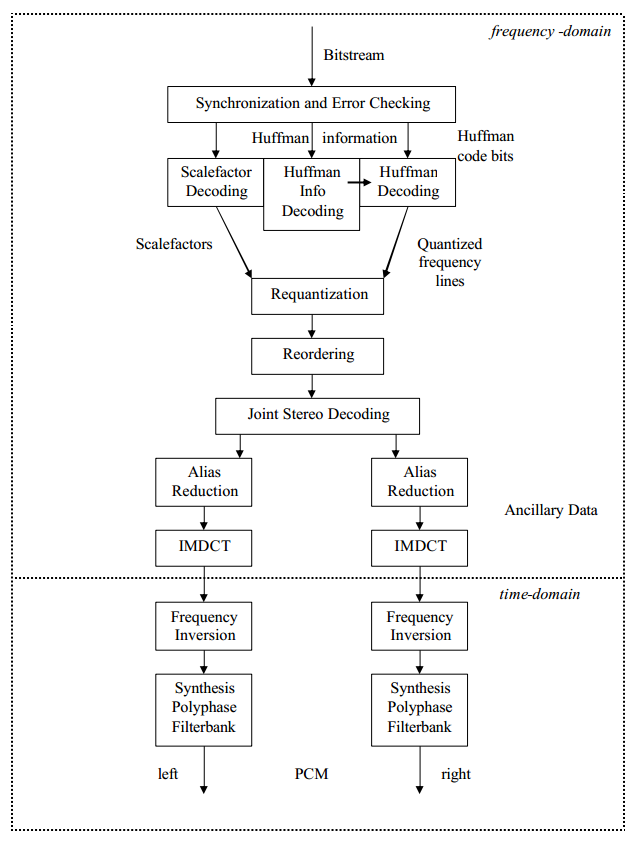
\includegraphics[scale=1]{decode_layout.png}
		\caption{Schema della decodifica MP3.}
		\label{fig:decode_layout}
	\end{figure}
	
	\section{Sincronizzazione} \label{sec:sincronizzazione}
		
		Il flusso di bit letti dal file \texttt{.mp3} viene scorso finhé non viene trovata la word di sincronizzazione (12 bit a 1). Se non viene rilevata la word di sincronizzazione di un frame, i dati non possono essere codificati ed il file è corrotto.
		
	\section{Decodifica Huffman e dei parametri relativi} \label{sec:decodifica_huffman}
		
		Innanzitutto è necessario decodificare i sample quantizzati tramite decodifica Huffman. Abbiamo visto che la codifica di Huffman è una codifica a lunghezza variabile ed inoltre dipende dalla tabella di Huffman impegata. Ad esempio non è possibile prendere una serie di bit a caso e sperare di decodificarli: è necessario leggere le sequenze codificate dall'inizio e sapere come sono stati codificati i dati. Vengono quindi decodificati (dalla Side Information) tutta una serie di parametri relativi alla codifica Huffman, come la suddivisione in regioni e sottoregioni, le tabelle di Huffman utilizzate, ecc \dots.\\
		Una volta in possesso di tutti i parametri necessari, i 576 sample verranno decodificati, utilizzando le tabelle di Huffman. Si noti che nel caso in cui meno di 576 sample siano trovati, dovranno essere inseriti i sample mancanti come sequenze di zeri.
		
	\section{Decodifica dei fattori di scala} \label{sec:decodifica_fattori_scala}
		
		In questa fase vengono decodificati i fattori di scala, che si trovano all'inizio dei dati principali di ogni granulo. I dati relativi a dove trovare i fattori di scala sono codificati nella Side Information di ogni granulo.
		
	\section{Riquantizzazione} \label{sec:riquantizzazione}
		
		Ricavando i valori di campi come global\_gain o scalefac\_scale si possono riquantizzare i sample quantizzati e scalati ottenuti dalla decodifica di Huffman, ottenendo le linee di frequenza generate dall'MDCT. I dati sui fattori di scala, necessari per la riquantizzazione, vengono forniti dallo step precedente (decodifica dei fattori di scala). Si osservi che in questo step vengono utilizzate funzioni di riquantizzazione differenti a seconda della finestra usata.
		
	\section{Riordinamento} \label{sec:riordinamento}
		
		Le linee di frequenza generate dal processo di riquantizzazione non sono sempre nell'ordine in cui dovrebbero essere dopo l'MDCT. Infatti se nell'MDCT era stata usata una finestra lunga, allora le linee di frequenza erano ordinate prima per sottobanda e poi per frequenza, mentre se erano state usate finestre corte erano ordinate per sottobanda, per finestra e quindi per frequenza. Tuttavia per aumentare l'efficienza della codifica Huffman, le linee di frequenza relative a finestre corte venivano riordinate, prima per sottobanda, poi per frequenza ed infine per finestra, in quanto sample di frequenza vicina hanno molto probabilmente un valore simile.\\
		Vengono allora cercate le linee di frequenza relative alle finestre corte in tutte le sottobande e, quando trovate, vengono riordinate, in modo da avere esattamente l'output dell'MDCT in fase di codifica.
		
	\section{Decodifica stereo} \label{sec:decodifica_stereo}
		
		Questo passaggio serve per separare l'insieme di sample generato in due segnali distinti: destro e sinistro. Per ricavare la modalità di canale utilizzata si leggo i valori dei campi Mode e Mode Extension dall'header del frame.
		
	\section{Riduzione dell'aliasing} \label{sec:riduzione_aliasing}
		
		Prima di invertire l'MDCT è necessario ridurre l'aliasing prodotto dal banco filtri di analisi. Questo viene fatto applicando una serie di 8 \textit{calcoli a farfalla} (si veda la Figura \ref{fig:butterfly}) per ogni sottobanda, che rimuovono gli artefatti dal segnale.
		
		\begin{figure}[h!]
			\centering
				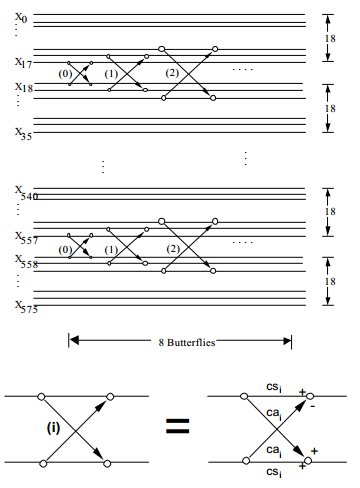
\includegraphics[scale=1]{butterfly.png}
			\caption{Riduzione dell'aliasing tramite calcoli a farfalla.}
			\label{fig:butterfly}
		\end{figure}
		
	\section{IMDCT} \label{sec:imdct}
		
		A questo punto è possibile applicare una \textit{IMDCT}, ovvero una \textit{Trasformata Discreta del Coseno Modificata Inversa}. L'IMDCT prende in input 576 linee di frequenza e restituisce 576 sample a dominio di tempo, suddivisi in 32 sottobande (18 sample per sottobanda).\\
		\\
		Analogamente alla (\ref{eqn:mdct}), la formula dell'IMDCT è la seguente:
		
		\begin{equation} \label{eqn:imdct}
			y_n = \frac{1}{N} \sum_{k=0}^{N-1}x_k\cdot\cos\left[\frac{\pi}{N}\left(n+\frac{1}{2}+\frac{N}{2}\right)\left(k+\frac{1}{2}\right)\right], \qquad n=0,\dots,2N-1.
		\end{equation}
		
	\section{Inversione di frequenza} \label{sec:inversione_frequenza}
		
		Dal momento che il banco filtri di analisi polifasico ha invertito le frequenze (similmente a quanto accade con la Trasformata di Fourier e sue derivate), per compensare si moltiplica ogni sample di indice dispari di ogni sottobanda dispari per $-1$.
		
	\section{Banco filtri di sintesi polifasico} \label{sec:banco_filtri_sintesi_polifasico}
		
		Infine, vengono fatti passare i sample di ogni sottobanda da un banco filtri di sintesi polifasico, che rappresenta l'inverso del banco filtri di analisi polifasico, visto in fase di codifica. Il risultato sono 576 sample PCM, per canale, che corrispondono al segnale audio decodificato.
	\chapter{Conclusioni} \label{chap:conclusioni}


	
	\nocite{*}
	\bibliographystyle{plainnat}
	\bibliography{biblio}
	
\end{document}